\chapter{Análise Bibliográfica sobre Simulação Multiagente para incêndios florestais, por Marcelo Aiache Postiglione\label{chap:bibliometria:marcelo3101}}

\section{Planejamento do estudo\label{FF@marcelo3101:questoes}}
O planejamento o  desenho do estudo deve descrever as motivações, questões de interesse, escopo, limitações e objetivos do trabalho. O planejamento do estudo deve motivar o tema escolhido e o interesse do autor.

Incêndios florestais se tornaram um objeto de estudo muito relevante. É possível perceber que florestas ao redor do mundo sofrem bastante com casos de incêndios. Um recente exemplo foi o caso da Austrália (\url{https://g1.globo.com/natureza/noticia/2020/07/28/incendios-na-australia-afetaram-3-bilhoes-de-animais-afirma-estudo.ghtml}) onde a vegetação e vários animais foram afetados pelas grandes queimas que ocorreram em 2020. Levando em consideração a importância dos diversos biomas a principal motivação para se realizar tais simulações seria para entender como a ignição ocorre e como o fogo se espalha nessas regiões de floresta.

No caso do meu trabalho, as perguntas que o nortearam foram:
\begin{itemize}
    \item O que pode se dizer sobre a produção científica global acerca desse assunto específico?  
    \item Como a simulação multiagente tem sido usada para compreender os fenômenos de ignição e espalhamento do fogo envolvidos nesses incêndios? 
    \item Quais são os principais conceitos ligados ao tema de pesquisa sobre incêndios florestais?
    \item Quais países que se destacam na pesquisa sobre simulações de incêndios florestais?
\end{itemize}

\subsection{O que já existe de pesquisa bibliométrica sobre esse tema?}

\cite{noauthor_forest-fire_2019} oferece uma boa explicação sobre o modelo matemático utilizado por esses estudos. É possível encontrar diversas pesquisas bibliométricas que realizam a análise sistemática sobre os modelos utilzados para simulações. \cite{noauthor_systematic_2022} é um exemplo de estudo que visa explorar os avanços realizados sobre o entendimento dos comportamentos dos incêndios florestais.

\subsection{Uso do Bibliometrix e Biblioshiny}
Serão usadas a ferramenta e o \textit{workflow} proposto pelos autores do pacote Bibliometrix, conforme indica a figura ~\ref{fig:bibliometrix:workflow}.

\subsection{Limitações} O exercício relatado foi feito em uma semana, envolvendo entre 5 a 10 horas de trabalho de cada autor.

Outros aspectos a reforçar:
\begin{itemize}
   
\item Deve-se fazer buscas na base de dados WoS ou SCOPUS;
\item é obrigatório declarar um conjunto de perguntas de pesquisa.
\item é preciso declarar o objetivo da pesquisa, que no caso da aqui relatada foi exercitar inicialmente, e relatar, o uso da técnica de análise bibliométrica, para fins didáticos.
\end{itemize}


\section{Coleta de dados\label{FF@marcelo3101:coleta}}

A coleta de dados feita usando o Web of Science (WoS) no dia 04 de dezembro de 2022, acessado por meio do Portal de Periódicos da CAPES.


\subsection{Query de Busca}

Foi usada a \query\  de busca ilustrada nas linhas 1 a 9 da listagem \ref{FF@marcelo3101:query}.

\lstinputlisting[numbers=left,basicstyle=\normalsize\ttfamily,caption={\query\  de busca sobre simulação multiagente de incêndios florestais, juntamente com processos de ignição e espalhamento do fogo.},label=FF@marcelo3101:query]
{exploratory-data-analysis/marcelo3101/PesqBibliogr/ForestFire/WoS-20221204/query.txt}

\subsubsection{Explicação para os termos de busca usados\label{MASSA:query}}

A busca consistiu de quatro cláusulas disjuntivas, unidas por uma conjunção \textit{and}, aplicadas à busca em \textit{all fields} (O termo de busca pode aparecer em qualquer área do artigo).

O termo \texttt{simul*} (linha 1 da query) foi utilizado para se obter artigos que realizem uso de simulações. 

Os termos \texttt{agent} e \texttt{multiagent},  (linha 3 da query) foram usados na segunda cláusula da \query\  para identificar os tipos de simulação desejados. Sendo esses baseados em agentes.

Os termos  \texttt{forest}, \texttt{jungle*}, \texttt{wood*}, \texttt{vegetation*} e \texttt{wild*}, na linha 5, foram usados em conjunção para recuperar apenas trabalhos que realizem simulações em regiões de florestas. 

A cláusula na linha 7 faz união entre o uso dos termos \texttt{fire}, \texttt{spread*}, \texttt{burn*} e \texttt{ignition}, para complementar a linha 5 e obter simulações sobre fogo, espalhamento do fogo e ignição em áreas florestais.

A cláusula localizada na linha 9,  antecedida pelo operador \texttt{NOT}, possui os termos \texttt{firefight*}, \texttt{extinguish*} e \texttt{decision} associados por disjunção e tem o objetivo de filtrar os resultados para retirar artigos que visam a simulação do combate ao fogo.

\subsection{Registros recuperados}

Os registros obtidos como resultado da busca encontram-se em \url{https://github.com/jhcf/Comput-Experim-20212-Overleaf2/exploratory-data-analysis/marcelo3101/PesqBibliogr/ForestFire/ WoS-20221204/wos366recs.txt}. 

Foram utilizadas as opções \textit{Exportar registros para arquivo de texto sem formatação} e \textit{export full record plus citations / exportar todas as informações, inclusive citações que realizam} no WoS, para que as citações também pudessem ser analisadas. Os 366 registros foram recuperados em uma única exportação, todos no mesmo arquivo de texto.

A listagem \ref{FF@marcelo3101:records} apresenta 93 linhas de um registro no formato RIS, referentes a um artigo recuperado da Web of Science. Cada um dos campos de um registro é marcado por um código de dois caracteres, nas colunas 1 e 2 de cada linha. Se a coluna está em branco repete-se o mesmo campo da linha anterior.
O significado de cada campo pode ser visto em \citep{wikipedia_ris_2017}.

Alguns campos específicos serão comentados a seguir:
\begin{description}
    \item [PT - Publication Type] indica o tipo da publicação, no caso específico um artigo de \textit{journal} (J);
    \item [AU - Author] Nome de um autor;
    \item [AF - Author Full Name] Nome completo de um autor;
    \item [TI - Title] Título da publicação;
    \item [SO - Source] Nome da revista;
    \item [DE - Descriptor] Palavras-chave;
    \item [AB - Abstract] Resumo;
    \item [CR - Cited Referente] Cada uma das referências citadas no artigo;
    \item [TC - Times Cited] Quantidade de vezes que esse artigo foi globalmente citado;
    \item [PY - Publication Year] Ano de publicação;
    \item [VL - Volume, IS - Issue] Volume e número onde o artigo foi publicado, na revista;
    \item [BP - Begin page, EP - End page] Páginas inicial e final do artigo dentro do volume e número da revista;
    \item [DI - Digital Object Identifier] Identificador único do artigo no sistema \url{http://doi.org};
    \item [DA - Date of Acquisition] Data em que o registro foi obtido da WoS;
    \item [ER - End of Record] Fim do registro.
\end{description}

\lstinputlisting[numbers=left,basicstyle=\tiny\ttfamily,caption={Exemplo do registro recuperado no formato RIS, sobre o tema simulação multiagente de incêndios florestais.},label=FF@marcelo3101:records]
{exploratory-data-analysis/marcelo3101/PesqBibliogr/ForestFire/WoS-20221204/assets/sampleris.txt}

\section{Análise dos dados\label{FF@marcelo3101:analise}}

\subsection{Filtragem de registros}
Antes da análise, é possível aplicar filtros sobre os registros obtidos.

Foi aplicado um filtro ao \dataset\   inicial, com 366 registros, que continham diversos tipos de registros. Foram mantidos apenas os registros de artigos publicados em revistas científicas\footnote{A suposição é que que o conhecimento de maior qualidade sobre o tema está nas publicações em revistas.}. Após a aplicação desse filtro, 359 registros foram mantidos no \dataset. Para esse capítulo, iremos chamá-lo de marcelo3101/ForestFire ou FF@marcelo3101

\subsection{Análise descritiva do \dataset\   FF@marcelo3101}

A análise bibliométrica descritiva faz uma descrição inicial do \dataset\  . Para explicação detalhada de como são calculadas as diversas taxas geradas pelo Bibliometrix veja a documentação do \textit{package} a partir da página \url{https://cran.r-project.org/web/packages/bibliometrix/index.html}. A análise bibliométrica descritiva é gerada pela função \texttt{biblioAnalysis}.

As informações mais gerais sobre o \dataset\   FF@marcelo3101 são as seguintes:
\begin{description}
    \item [\textit{Timespan}] Os artigos que atenderam aos critérios de busca e filtragem foram publicados a partir de 1993, até 2022. Ou seja, não foram encontrados registros entre 1945 e 1992.
    \item [\textit{Sources (Journals, Books, etc)}] São 269 fontes de informação que publicaram os documentos que estão presentes no \dataset\   FF@marcelo3101. Ou seja, cada fonte publicou, em média, $359/269=1,33$ artigo. \footnote{Note que a média, enquanto medida de tendência central, pode não ser a que melhor reflete a tendência a quantidade de artigos publicados por revista.}
    \item [\textit{Average years from publication}] A média do tempo de publicação dos artigos no \dataset\   FF@marcelo3101 é de 7,58 anos.
    \item [\textit{Average citations per documents}] Cada artigo no \dataset\   FF@marcelo3101 foi citado, em média 30,69 vezes\footnote{Note que a média, enquanto medida de tendência central, pode não ser a que melhor reflete a tendência de  citações a artigos.}.
    \item [\textit{Average citations per year per doc}] Após publicado, cada um dos 359 artigos do \dataset\   FF@marcelo3101  foi citado 2,5 vezes por ano, em média.
    \item [\textit{References}] O \dataset\  FF@marcelo3101 contém 19240 referências citadas (tags CR).
    \item [\textit{Keywords Plus (ID)}] 1755 distintas palavras-chave do tipo Keywords Plus (ID)\footnote{\textit{KeyWords Plus} são ``termos de índice gerados automaticamente a partir dos títulos de artigos citados. Os termos do KeyWords Plus devem aparecer mais de uma vez na bibliografia e são ordenados de frases com várias palavras a termos únicos. O KeyWords Plus aumenta o número de resultados tradicional de palavras-chave ou títulos.'' Fonte: \url{https://images.webofknowledge.com/WOKRS410B4/help/pt_BR/WOS/hp_full_record.html}} foram encontradas no \dataset\   FF@marcelo3101. 
    \item [\textit{Author's Keywords (DE)}] 1473 distintas palavras-chave indicadas pelos autores foram encontradas no \dataset\  .
    \item [\textit{Authors}] 1641 distintos nomes de autores foram encontrados no \dataset\  \footnote{Um mesmo autor pode ter uma ou mais diferentes grafias no \dataset\  , e serão reconhecidos dois ou mais autores diferentes, embora de fato sejam apenas um. Isso significa que a quantidade de \textbf{nomes de autores} equivale à quantidade de \textbf{autores}. Adicionalmente, é possível que distintos autores sejam reconhecidos com o mesmo nome, isso é, que sejam homônimos. Ou seja, o \dataset\   em geral conterá erros de contagem na quantidade de autores reais.}.
    \item [\textit{Author Appearances}] Os 1641 distintos (nomes de) autores foram encontrados 1755 vezes, como autores de artigos.
    \item [\textit{Authors of single-authored documents}] Dentre os 1641 distintos (nomes de) autores encontrados, 22 deles editaram artigos individualmente, isso é, sem co-autores.
    \item [\textit{Authors of multi-authored documents}] Dentre os 1641 distintos (nomes de) autores encontrados, 1619 deles editaram artigos com um ou mais co-autores"
    \item [\textit{Single-authored documents}] Dentre os 359 documentos presentes no \dataset\   FF@marcelo3101, 22 foram escritos por um único autor, e os 337 restantes foram elaborados em co-autoria.
    \item [\textit{Documents per Author}] Dentre os 1641 distintos (nomes de) autores, cada um publicou em média 0,218 artigos.
    \item [\textit{Authors per Document}] Cada um dos 359 documentos presentes no \dataset\   FF@marcelo3101 foi autorado com 4,57 autores em média ($1641 / 359 = 4,57$).
    \item [\textit{Co-Authors per Documents}] Temos uma média de 4,89 co-autores por registro para os 359 documentos do \dataset\   FF@marcelo3101.
    \item [\textit{Collaboration Index}] Os 1619 (nomes de) autores que editaram artigos com um ou mais co-autores, colaboraram em media 4,50 vezes para editar os 359 artigos elaborados em co-autoria, gerando, assim, um índice de colaboração 4,50. 
\end{description}



\subsection{Evolução da Produção Científica}

\begin{figure}
    \centering
    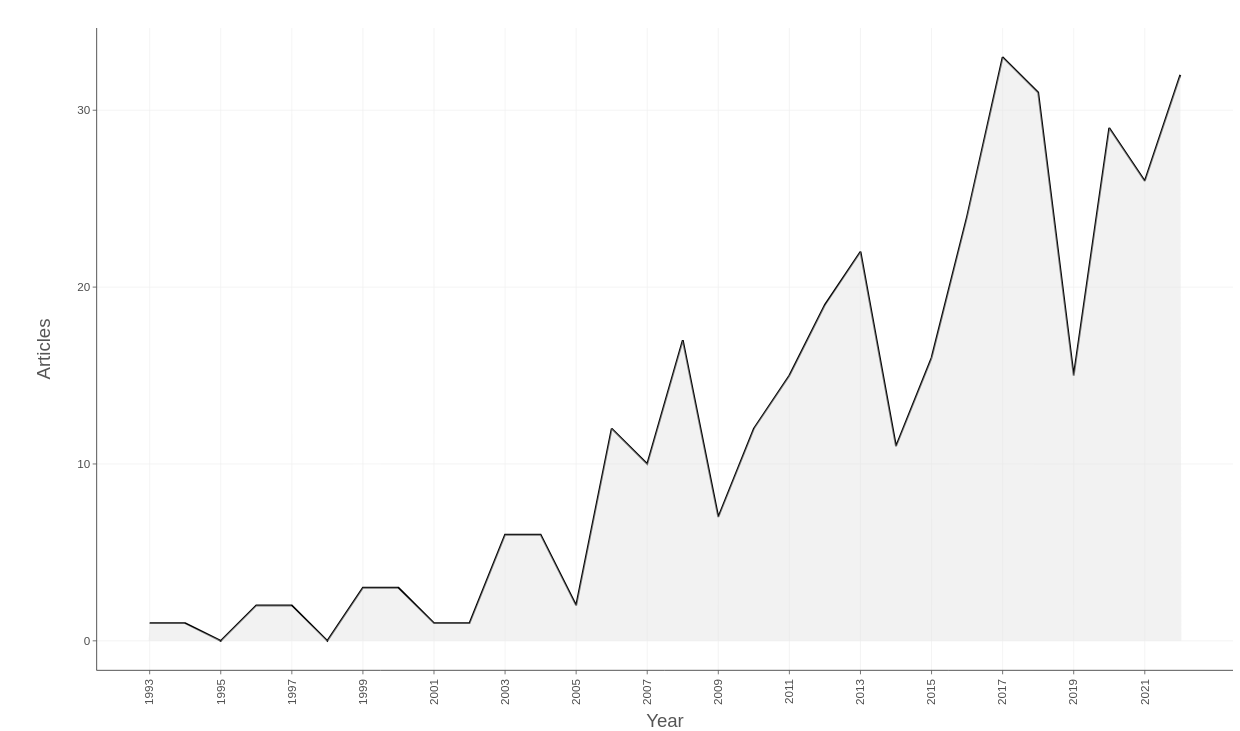
\includegraphics[width=1\textwidth]{exploratory-data-analysis/marcelo3101/PesqBibliogr/ForestFire/WoS-20221204/assets/AnnualScientificProductionFFMarcelo3101.png}
    \caption{Evolução da produção científica no \dataset\   FF@marcelo3101.}
    \label{fig:evol:anual:FF@marcelo3101}
\end{figure}

A figura \ref{fig:evol:anual:FF@marcelo3101} apresenta a evolução da produção científica mundial no tema de interesse, segundo o \dataset\   FF@marcelo3101. A curva mostra uma tendência de crescimento aproximadamente exponencial da quantidade de publicações, desde a primeira identificada em 1990.

O \textit{Annual Growth Rate} do \dataset\   é de 12,69\%, bem maior que a taxa média de crescimento da publicação científica mundial, de cerca de 3,3\% anuais, em 2016, como ilustra o estudo em \url{https://www.researchgate.net/publication/333972683_Dynamics_of_scientific_production_in_the_world_in_Europe_and_in_France_2000-2016}, página 23.

\subsection{Interpretação do Crescimento} A elevada taxa de crescimento do \dataset\  FF@marcelo3101, indica que o tema é um grande foco de estudo. Um dos fatores que pode colaborar para isso é o fato de grandes incêndios terem acontecido recentemente, vide caso da Austrália que em 2020 sofreu com enormes queimadas. Além dos danos causados à flora e à fauna de regiões afetadas por queimadas o que torna a análise e simulação desses incêndios bem relevante.

\subsection{Evolução das Citações}

\begin{figure}
    \centering
    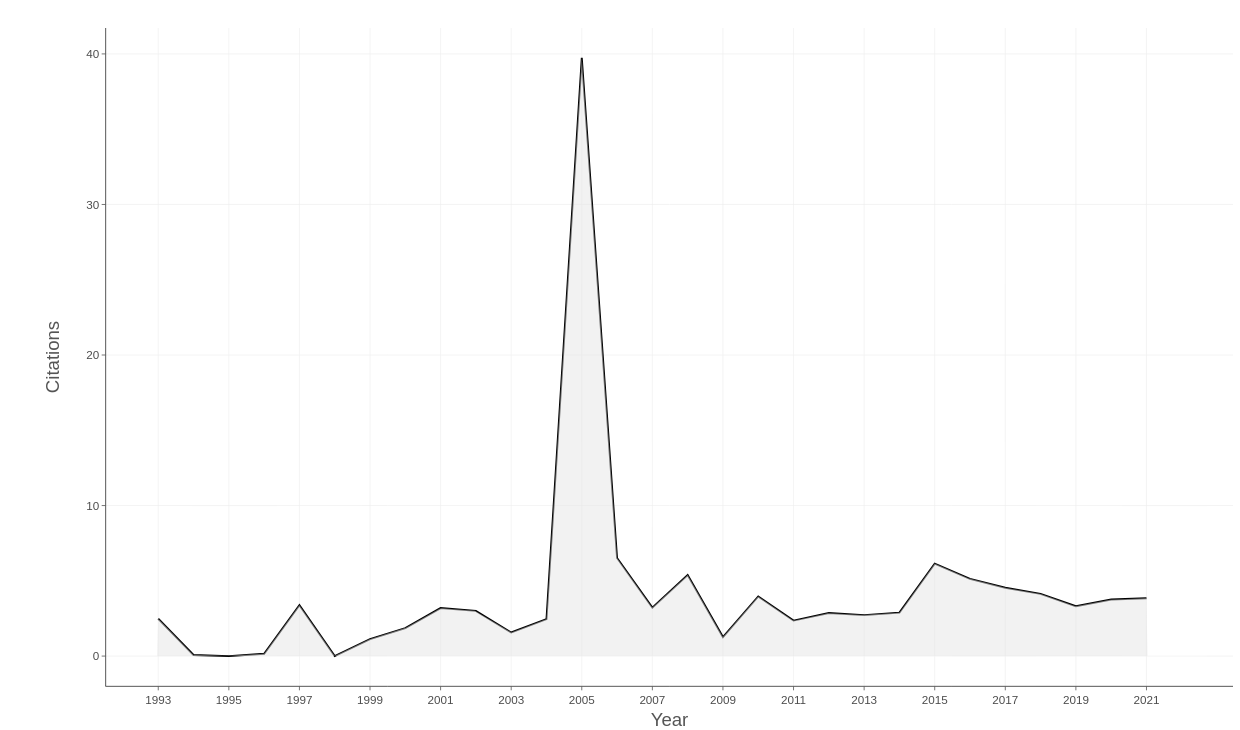
\includegraphics[width=1\textwidth]{exploratory-data-analysis/marcelo3101/PesqBibliogr/ForestFire/WoS-20221204/assets/averageCitationPerYearFFmarcelo3101.png}
    \caption{Evolução das citações ao \dataset\   FF@marcelo3101.}
    \label{fig:evol:anual:citacoes:FF@marcelo3101}
\end{figure}

A figura \ref{fig:evol:anual:citacoes:FF@marcelo3101} apresenta a evolução da média de citações aos 359 artigos no \dataset\   FF@marcelo3101. 
No geral, temos uma grande estabilidade. O pico que aparece nos anos de 2005 e 2006 deve-se, possivelmente, ao grande número de incêndios florestais ocorridos na Califórnia (Fonte: \url{https://en.wikipedia.org/wiki/2005_California_wildfires} e \url{https://en.wikipedia.org/wiki/2006_California_wildfires}). Um fato intrigante é que apesar dos grandes incêndios que ocorreram na Austrália em 2019 e em 2020, o dataset manteve um comportamento considerado típico. \footnote{Note que o cálculo do número  médio de citações, nesse caso, utiliza os valores computados no tag "TC (Times Cited)", já presentes no \dataset\   obtido. Ou seja, o gráfico baseia-se no número de citações globais (externas ao \dataset\   FF@marcelo3101), e não no número de citações locais (citações a um artigo do \dataset\   feitas por alguns dos outros artigos dentro do próprio \dataset).}.

\subsection{Interpretação das Citações}
Apesar do grande pico, podemos perceber um comportamento mais estável para as citações globais dos artigos presentes no \dataset\.

\subsection{\textit{Three-Field Plots (Sankey diagram)} \label{FF@marcelo3101:Sankey}}

\begin{figure}
    \centering
    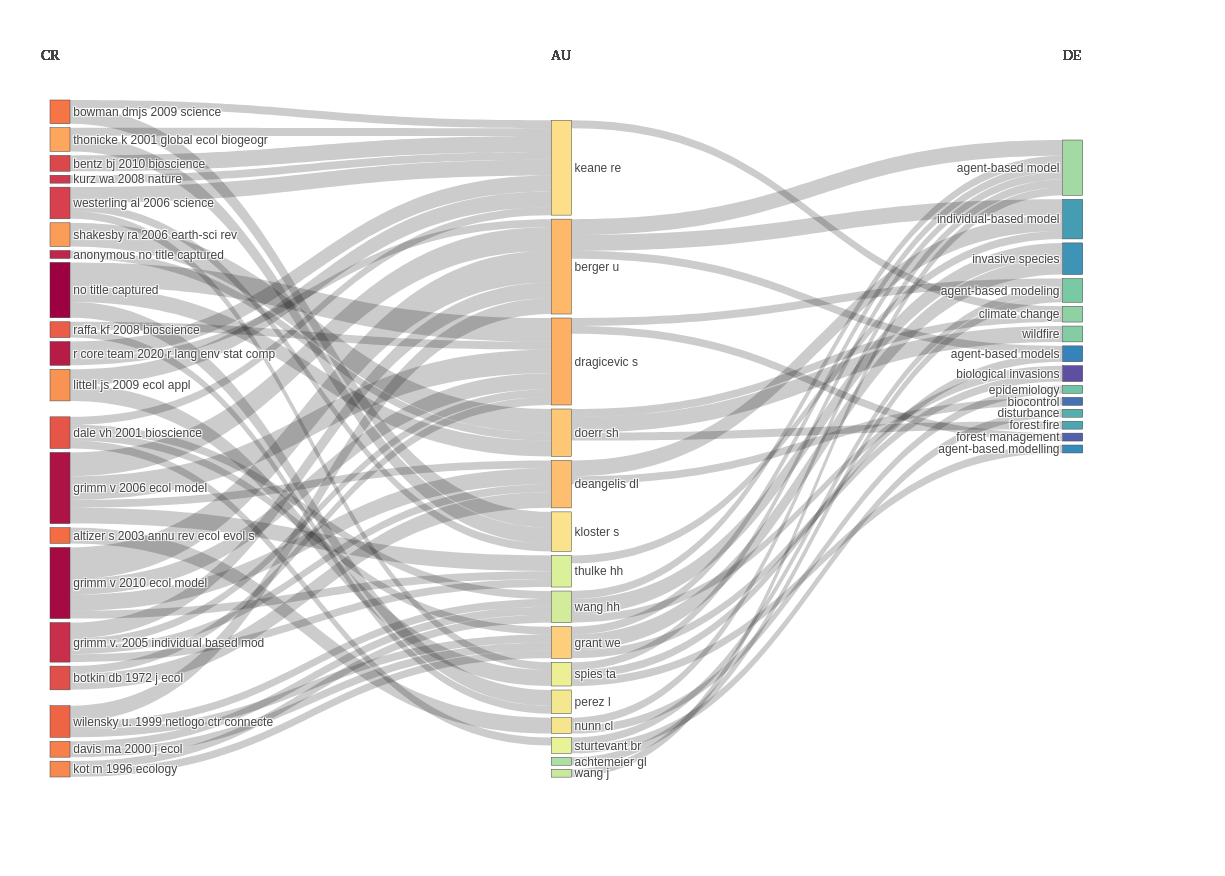
\includegraphics[angle=0,width=1\textwidth]{exploratory-data-analysis/marcelo3101/PesqBibliogr/ForestFire/WoS-20221204/assets/threeFieldPlotFFmarcelo3101.png}
    \caption{Plotagem ``Três Campos'' (Sankey plot) do \dataset\   FF@marcelo3101: 20 Autores, Citações e Palavras-Chave mais proeminentes.}
    \label{fig:FF@marcelo3101:ThreeFieldPlot}
\end{figure}

A figura \ref{fig:FF@marcelo3101:ThreeFieldPlot} apresenta a plotagem do tipo ``Três Campos'' do \dataset\   FF@marcelo3101, vinculando, ao centro, os 20 Autores mais proeminentes (AU), à esquerda, as 20 Citações mais frequentes (CR - Cited Records), e à direita, as 20 Palavras-Chave mais frequentes empregadas pelos autores.

\subsection{Interpretação da figura \ref{fig:FF@marcelo3101:ThreeFieldPlot}}

Dos vinte autores mais relevantes, citados pelos artigos do \dataset\ FF@marcelo3101, e das palavras-chave mais relevantes, temos um domínio norte-americano e europeu. Esse padrão também se mantém para as citações.

Possuímos alguns termos dentre as palavras-chave (DE) que não estão diretamente relacionados ao interesse central da busca realizada. Esses termos são \textbf{Invasive species} e \textbf{Biological invasions}.

Pela interpretação da plotagem da figura \ref{fig:FF@marcelo3101:ThreeFieldPlot}, observa-se que a maioria dos artigos mais citados encontram-se publicados entre os anos 2000 e 2010. Indicando que, na década seguinte, nenhum trabalho obteve o mesmo impacto, exceto por um registro de 2020. 

\subsubsection{Autores mais relevantes\label{FF@marcelo3101:Sankey:AutoresRelevantes}}

Algumas considerações sobre os trabalhos mais citados.

\begin{itemize}
    \item  \cite{bowman_fire_2009} Discute os maiores problemas envolvidos sobre o processo de entendimento do papel do fogo no globo terrestre. Abordando desde os primeiros contatos feitos pelos homens e registrados até grandes incêncios e acidentes;
    \item  O artigo de Thonicke; KVenevsky, S; Sitch, S e Cramer, W; Explora a simulação da influência do fogo no equilíbrio dinâmico de vegetações em escala global;
\end{itemize}

O Segundo artigo citado está presente no dataset.

%\subsection{Análises Bibliométricas: Fontes de Informação}

%\begin{figure}
%    \centering
%    \includegraphics[angle=0,width=1\textwidth]{}
%    \caption{Plotagem ``Três Campos'' (Sankey plot) do dataset MASSA@jhcf: 20 Autores, Citações e Palavras-Chave mais proeminentes.}
%    \label{fig:MASSA@jhcf:ThreeFieldPlot}
%\end{figure}

\subsection{Citações globais aos artigos no \dataset}

A tabela \ref{table:FF@marcelo3101:MostGlobalCitedDocs} apresenta a lista dos 10 artigos do \dataset, que foram mais citados, ordenados de forma decrescente pelo número global de citações do artigo, nos índices da WoS. Para ada artigo é apresentada a referencia abreviada, o DOI e a quantidade de vezes que ele foi citado globalmente (no índice do WoS).

\begin{table}[htp]
\centering
\resizebox{\textwidth}{!}{%
\begin{tabular}{|l|l|l|l|l|}
\hline
Paper                                 & DOI                                & Total Citations & TC per Year & Normalized TC \\ \hline
GRIMM V, 2005, SCIENCE                & 10.1126/science.1116681            & 1339            & 74.39       & 1.98          \\ \hline
LAIRD DA, 2008, AGRON J               & 10.2134/agronj2007.0161            & 599             & 39.93       & 7.94          \\ \hline
THOM D, 2016, BIOL REV                & 10.1111/brv.12193                  & 344             & 49.14       & 11.17         \\ \hline
ALONGI J, 2015, PROG POLYM SCI        & 10.1016/j.progpolymsci.2015.04.010 & 323             & 40.38       & 7.51          \\ \hline
BEARD RW, 2006, P IEEE                & 10.1109/JPROC.2006.876930          & 303             & 17.82       & 2.91          \\ \hline
SZWAJA S, 2010, FUEL                  & 10.1016/j.fuel.2009.08.043         & 283             & 21.77       & 5.95          \\ \hline
OGDEN NH, 2006, INT J PARASITOL       & 10.1016/j.ijpara.2005.08.016       & 256             & 15.06       & 2.46          \\ \hline
CERDA A, 2008, CATENA                 & 10.1016/j.catena.2008.03.010       & 247             & 16.47       & 3.27          \\ \hline
SHI DS, 2006, J PHARMACOL EXP THER    & 10.1124/jpet.106.111807            & 214             & 12.59       & 2.05          \\ \hline
TINAUT FV, 2008, FUEL PROCESS TECHNOL & 10.1016/j.fuproc.2008.04.010       & 162             & 10.80       & 2.15 \\ \hline  
\end{tabular}%
}
\caption{Tabela com os 10 artigos mais citados globalmente no \dataset\  FF@marcelo3101}
\label{table:FF@marcelo3101:MostGlobalCitedDocs}
\end{table}

Os artigos estão relacionados ao tema e são usados para a elaboração dos artigos que realizam as simulações.

\subsection{Espectroscopia das referências}

A técnica de espectroscopia das referências bibliográficas (``reference publication year spectroscopy'' (RPYS)) de um \dataset\cite{marx_detecting_2014} possibilita identificar as raízes históricas  de um campo de conhecimento. 

A figura \ref{fig:FF@marcelo3101:ReferenceSpectroscopy} apresenta, distribuída ao longo do tempo, a quantidade de referências citadas no \dataset\, para cada ano, bem como os desvios dessa quantidade em relação à média (em vermelho). 

A mais antiga das referências usadas é do ano de 1732, e segue com certa estabilidade. O comportamento se altera bruscamente e o comportamento da linha vermelha entre os anos de 2005 e 2011 indica um grande aumento. Esse pico na média de citações, possivelmente ocorreu devido aos incêndios ocorridos na califórnia que aumentaram a produção e interesse científico sobre o assunto.

\begin{figure}
    \centering
    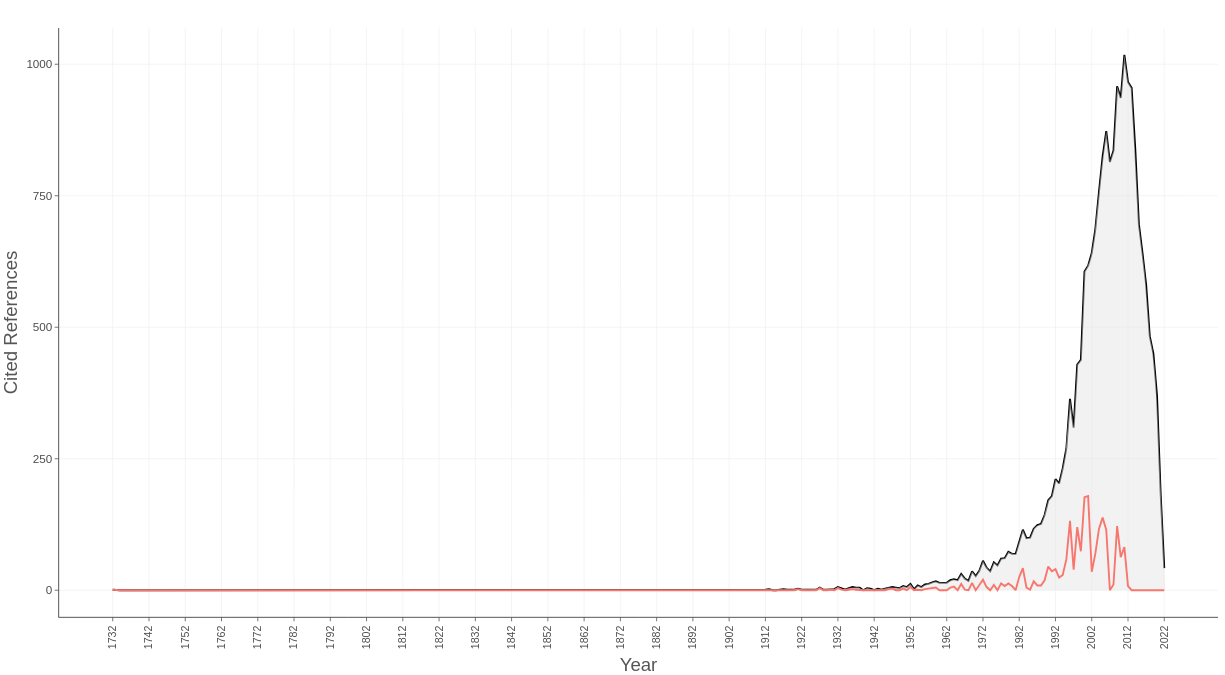
\includegraphics[width=1\textwidth]{exploratory-data-analysis/marcelo3101/PesqBibliogr/ForestFire/WoS-20221204/assets/ReferenceSpectroscopyFFmarcelo3101.png}
    \caption{Espectroscopia (RPYS) completa das referências do \dataset\ FF@marcelo3101.}
    \label{fig:FF@marcelo3101:ReferenceSpectroscopy}
\end{figure}

\subsection{Uso de palavras dentro dos artigos no \dataset}

As últimas das métricas aplicadas a documentos, disponíveis para aplicação no Bibliometrix é baseada na ocorrência de termos no texto dos documentos. A mais comum delas é baseada na simples contagem de frequência das palavras, como ilustra a figura \ref{fig:FF@marcelo3101:Word:Occurrences}, com os 10 termos mais frequentes em uso.

\begin{figure}
    \centering
    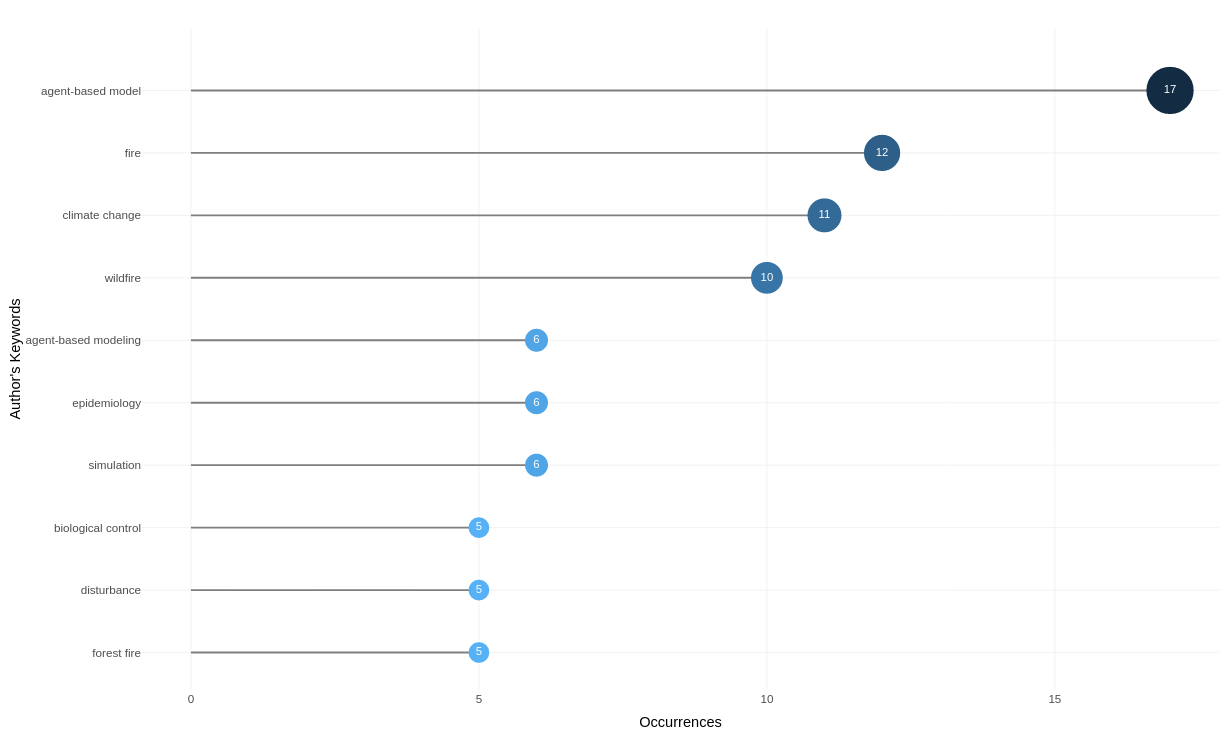
\includegraphics[width=1\textwidth]{exploratory-data-analysis/marcelo3101/PesqBibliogr/ForestFire/WoS-20221204/assets/MostFrequentWordsFFmarcelo3101.png}
    \caption{10 palavras (termos) mais frequentes no \dataset\ FF@marcelo3101.}
    \label{fig:FF@marcelo3101:Word:Occurrences}
\end{figure}

Outras formas de apresentação alternativas são apresentadas nas duas figuras a seguir, que ilustram de forma diferente a mesma informação, como em:
\begin{description}
    \item [Word Cloud] Uma nuvem de palavras, na figura \ref{fig:FF@marcelo3101:WordCloud-100words}, com evidencias para as 50 palavras mais frequentes;
    \item [Tree Map] Um mapa em árvore, na figura \ref{fig:FF@marcelo3101:TreeMap}, com evidências para as 50 palavras mais frequentes;
\end{description}

\begin{figure}
    \centering
    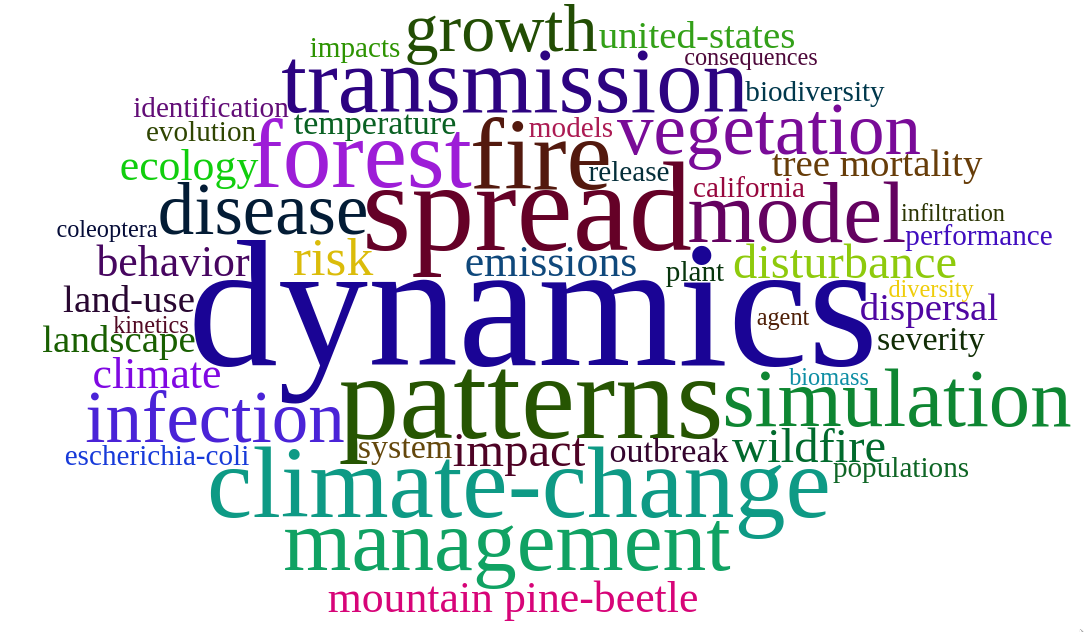
\includegraphics[width=1\textwidth]{exploratory-data-analysis/marcelo3101/PesqBibliogr/ForestFire/WoS-20221204/assets/WordCloudFFmarcelo3101.png}
    \caption{Nuvem dos 50 termos mais frequentes do \dataset\ FF@marcelo3101.}
    \label{fig:FF@marcelo3101:WordCloud-100words}
\end{figure}

\begin{figure}
    \centering
    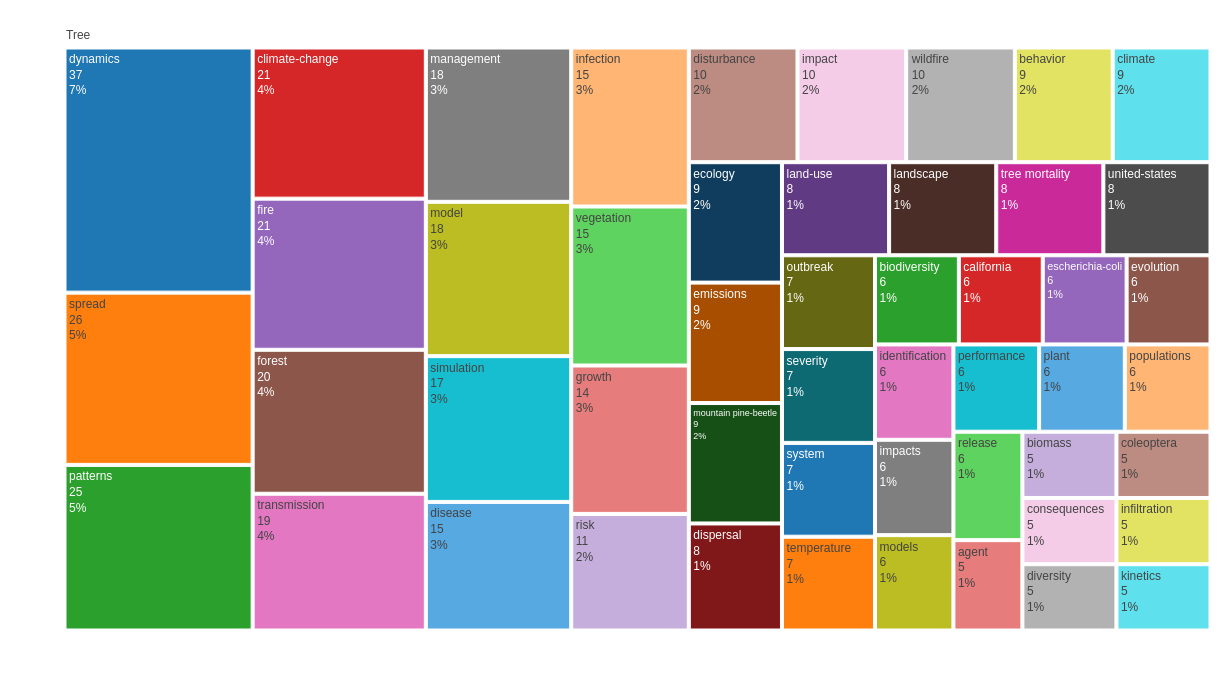
\includegraphics[width=1\textwidth]{exploratory-data-analysis/marcelo3101/PesqBibliogr/ForestFire/WoS-20221204/assets/TreeMapFFmarcelo3101.png}
    \caption{\textit{Tree Map} dos 50 termos mais frequentes do \dataset\ FF@marcelo3101.}
    \label{fig:FF@marcelo3101:TreeMap}
\end{figure}

Por fim, o Bibliometrix permite apresentar o uso dos termos ordenado temporalmente, como nas duas figuras a seguir:

\begin{description}
    \item [Word Growth / Word Dynamics] que mostra o crescimento de uso das palavras mais frequentes, como na figura \ref{fig:FF@marcelo3101:WordDynamics};
    \item [Trending topics] que mostra as tendências para uso de determinadas palavras em determinadas faixas de tempo, como em \ref{fig:FF@marcelo3101:TrendTopics}. Para obtenção do gráfico foram determinados os seguintes valores para os parâmetros: frequência mínima de ocorrência para que um termo seja considerado = 15, quantidade máxima de tópicos por ano = 7.
\end{description}

\begin{figure}
    \centering
    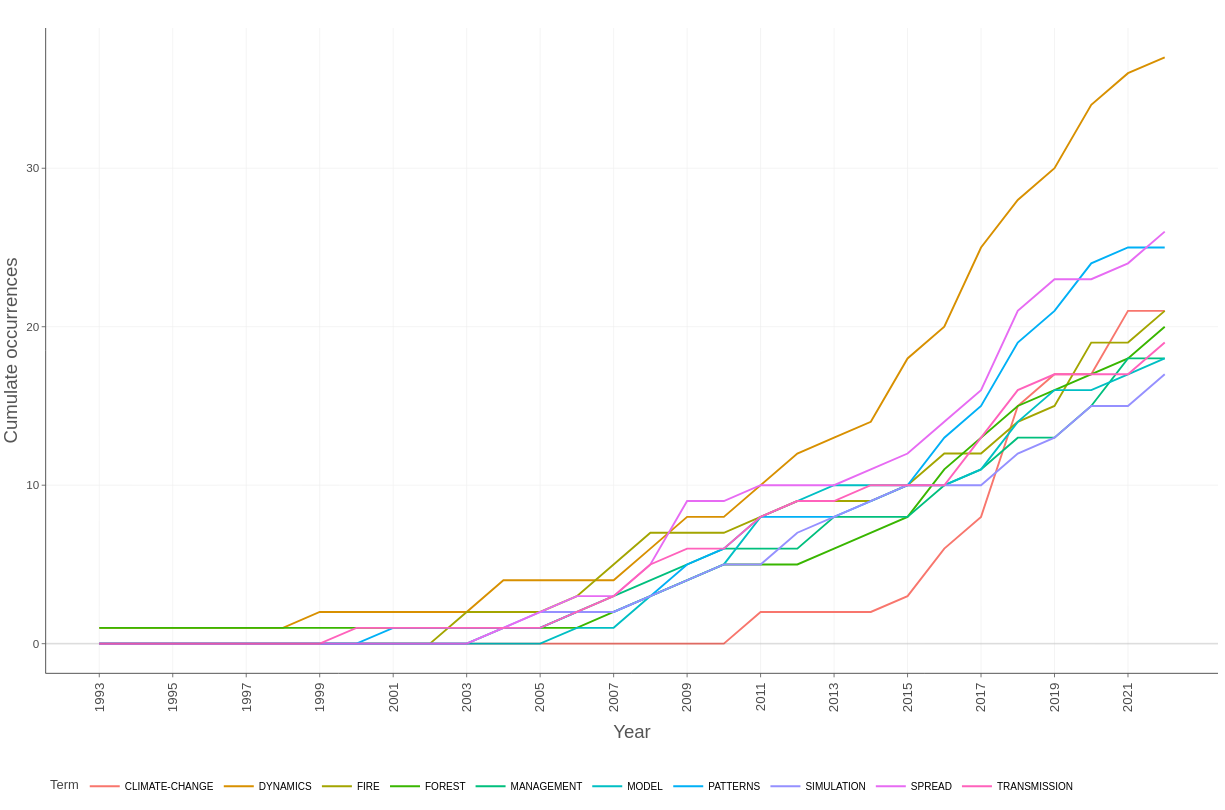
\includegraphics[width=1\textwidth]{exploratory-data-analysis/marcelo3101/PesqBibliogr/ForestFire/WoS-20221204/assets/WordDynamicsFFmarcelo3101.png}
    \caption{Dinâmica de uso ao longo do tempo, dos 10 termos mais frequentes do \dataset\ FF@marcelo3101.}
    \label{fig:FF@marcelo3101:WordDynamics}
\end{figure}

\begin{figure}
    \centering
    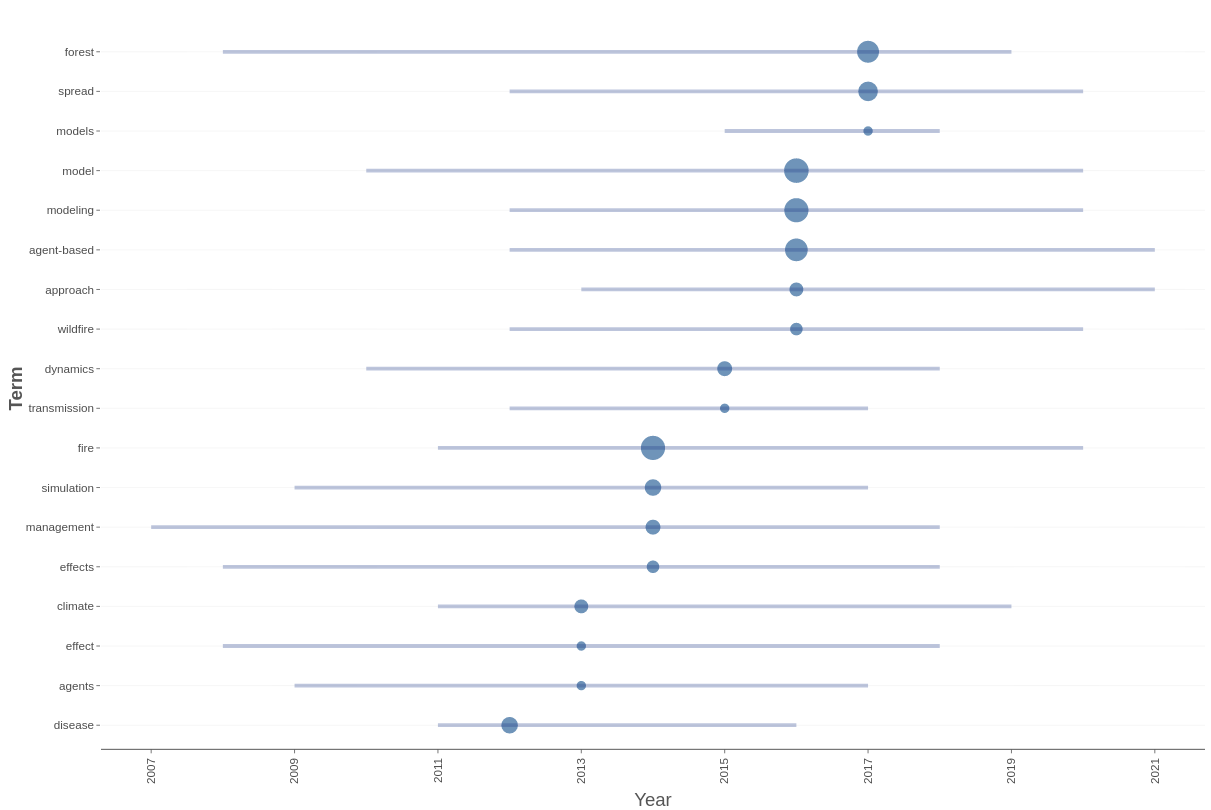
\includegraphics[width=1\textwidth]{exploratory-data-analysis/marcelo3101/PesqBibliogr/ForestFire/WoS-20221204/assets/TrendTopicsFFmarcelo3101.png}
    \caption{\textit{Trending Topics} do \dataset\ FF@marcelo3101, WF = 15, WPY=7.}
    \label{fig:FF@marcelo3101:TrendTopics}
\end{figure}

\subsection{Autores mais produtivos no \dataset}

A figura \ref{fig:FF@marcelo3101:Author:Production} apresenta a lista ordenada e decrescente dos autores com maior número de artigos no \dataset.

\begin{figure}
    \centering
    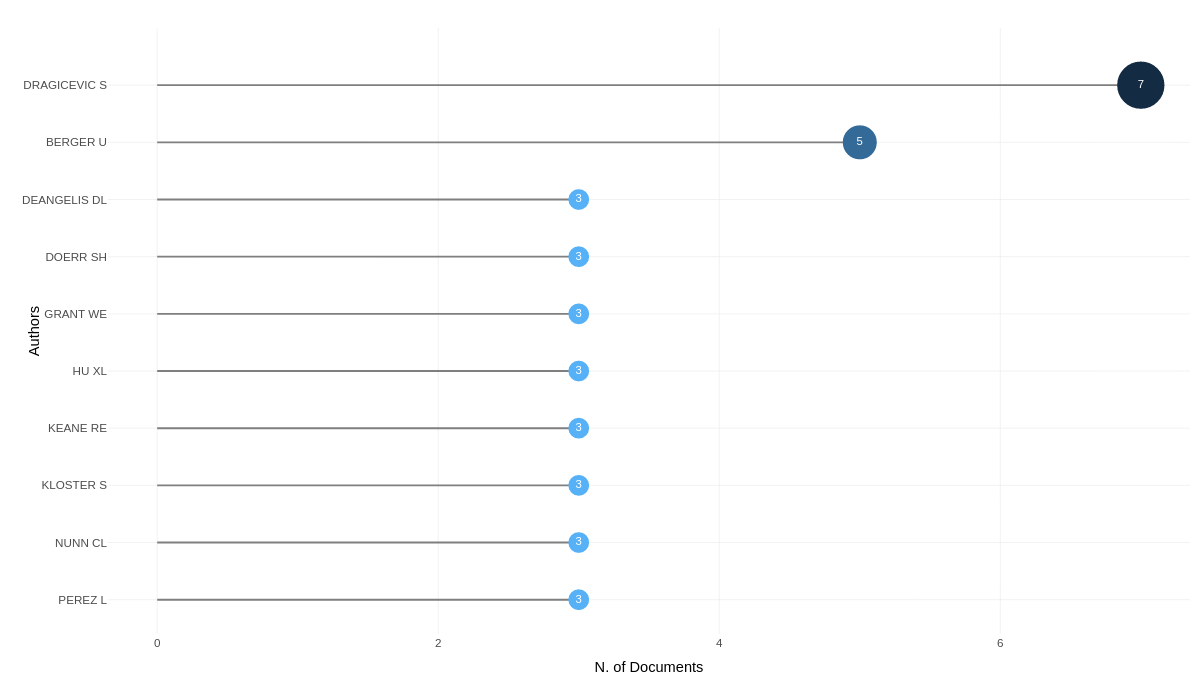
\includegraphics[width=1\textwidth]{exploratory-data-analysis/marcelo3101/PesqBibliogr/ForestFire/WoS-20221204/assets/mostRelevantAuthorFFmarcelo3101.png}
    \caption{10 autores com mais artigos no \dataset\ FF@marcelo3101.}
    \label{fig:FF@marcelo3101:Author:Production}
\end{figure}

\subsection{Autores mais relevantes localmente citados}

A figura \ref{fig:FF@marcelo3101:Author:LocalProduction} apresenta a lista ordenada e decrescente dos autores com maior número de artigos citados por outros artigos no \dataset. Provavelmente são os autores mais impactantes para a atual forma do \dataset\ FF@marcelo3101.

\begin{figure}
    \centering
    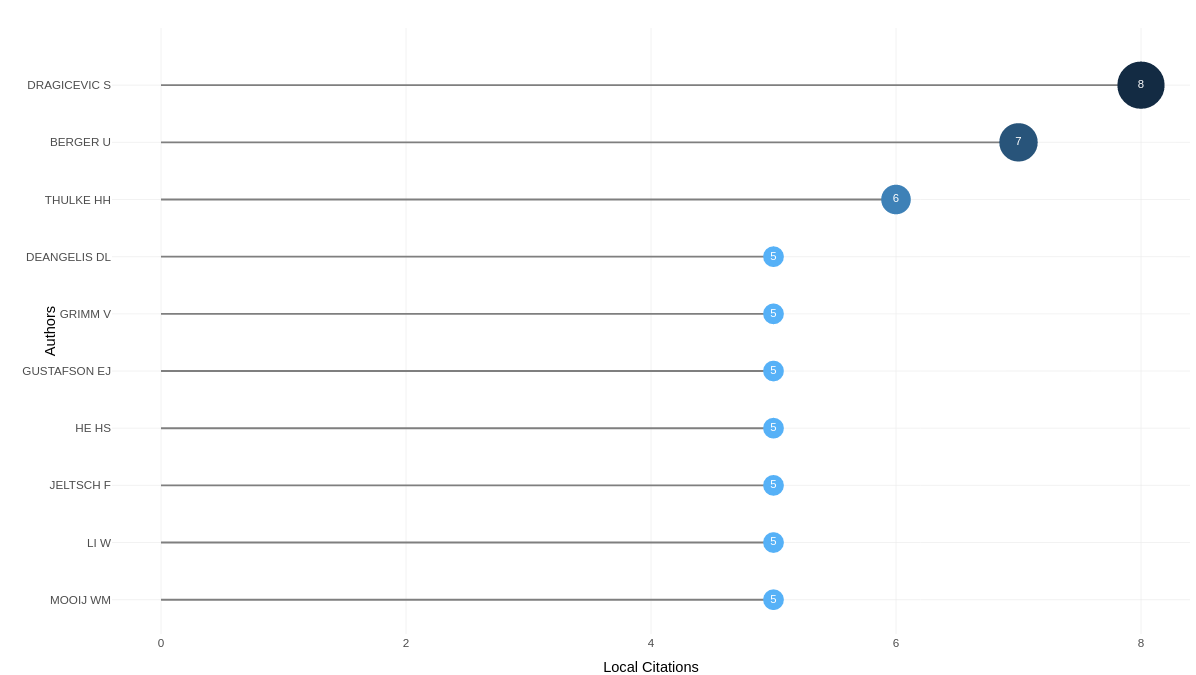
\includegraphics[width=1\textwidth]{exploratory-data-analysis/marcelo3101/PesqBibliogr/ForestFire/WoS-20221204/assets/MostLocalCitedAuthorsFFmarcelo3101.png}
    \caption{10 autores com mais artigos citados por outros artigos no \dataset\ FF@marcelo3101.}
    \label{fig:FF@marcelo3101:Author:LocalProduction}
\end{figure}

\subsubsection{Variação da produtividade dos autores ao longo do tempo}

Os cientistas passam por períodos mais ou menos produtivos.
Diagramas como o da figura \ref{fig:FF@marcelo3101:Author:TopAuthorsProductionOverTime} apresentam essas fases, em relação ao \dataset\ FF@marcelo3101.

\begin{figure}
    \centering
    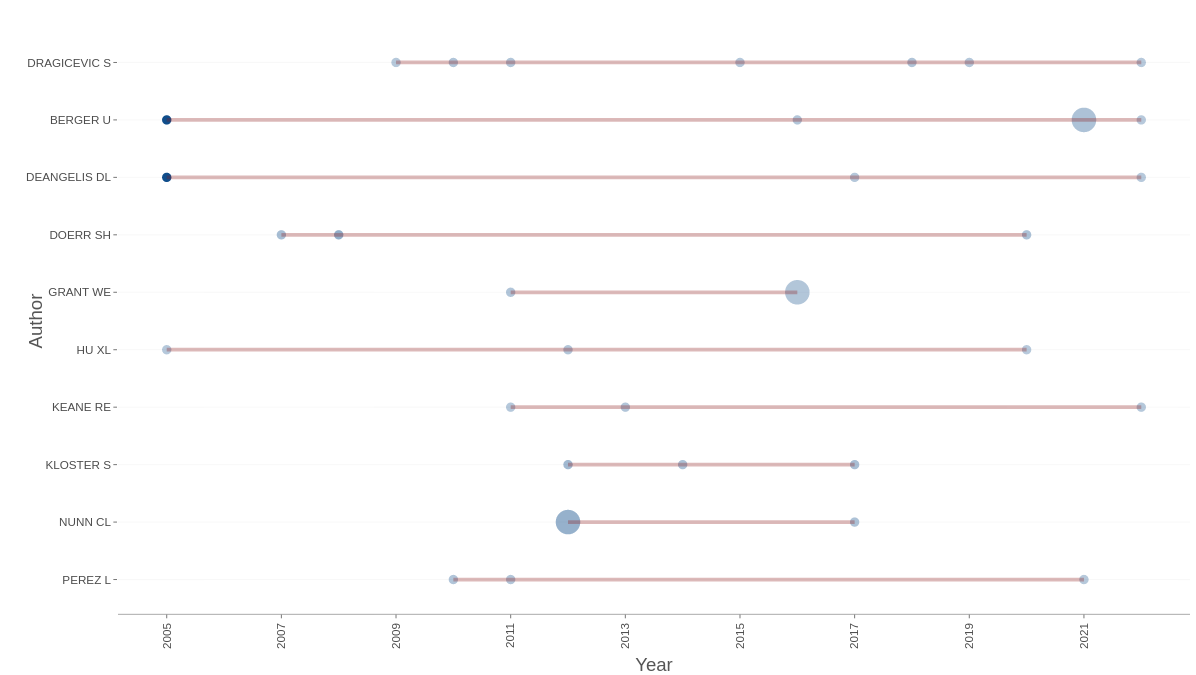
\includegraphics[width=1\textwidth]{exploratory-data-analysis/marcelo3101/PesqBibliogr/ForestFire/WoS-20221204/assets/AuthorsProductionOverTimeFFmarcelo3101.png}
    \caption{Variação da produção dos autores de maior impacto, do \dataset\ FF@marcelo3101.}
    \label{fig:FF@marcelo3101:Author:TopAuthorsProductionOverTime}
\end{figure}

\subsection{Lei de Lotka}

A Lei de Lotka (ver \url{https://en.wikipedia.org/wiki/Lotka\%27s_law}) estabelece uma distribuição de frequência aproximadamente inversamente quadrática ou cúbica, para o número de artigos publicados pelos autores de qualquer área do conhecimento. Isso é, se 1000 pessoas publicam ao longo de sua contribuição para o campo de conhecimento apenas um documento, então
entre $1000/x^{2}$ a $1000/x^{3}$ publicam $x$ documentos. Ou seja, entre
$1000/2^{2}$ a $1000/2^{3}$ pessoas publicam dois documentos, $1000/3^{2}$ a $1000/3^{3}$ pessoas publicam três documentos etc.

Se os dados empíricos do \dataset\ são alinhados à essas curvas, então é correto supor que o \dataset\ é bem formado. Podemos verificar que há uma aproximação satisfatória na figura \ref{fig:FF@marcelo3101:Author:Lotka}.

\begin{figure}
    \centering
    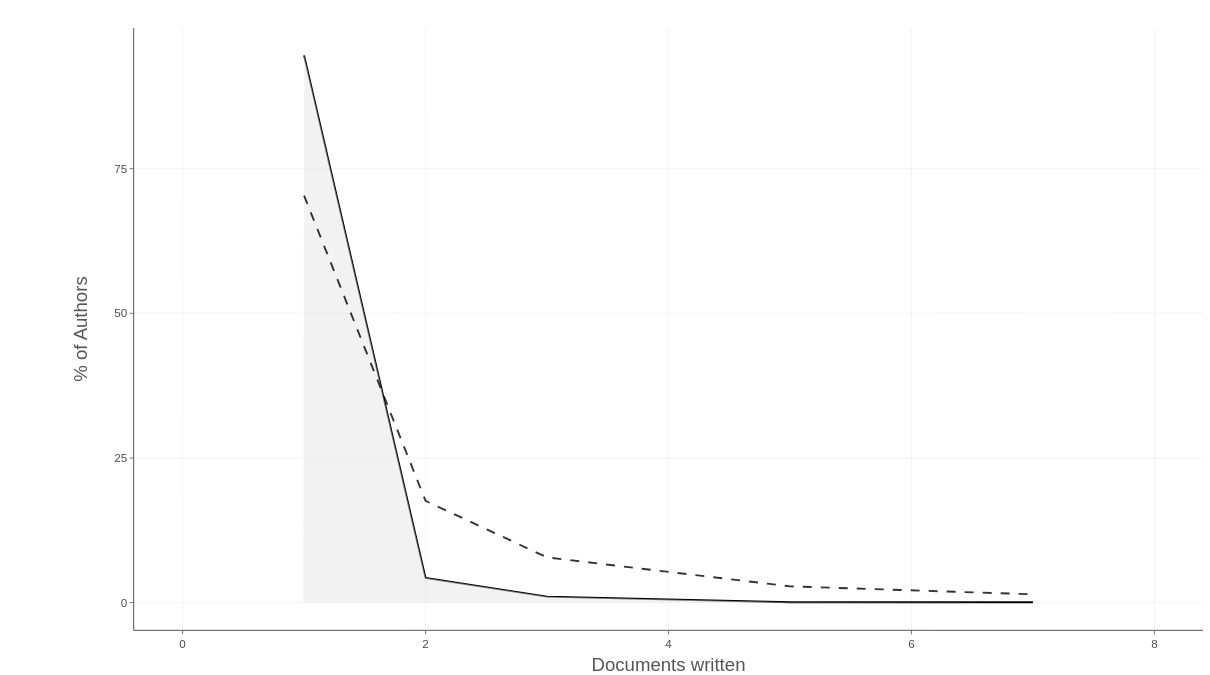
\includegraphics[width=1\textwidth]{exploratory-data-analysis/marcelo3101/PesqBibliogr/ForestFire/WoS-20221204/assets/LoktasLawFFmarcelo3101.png}
    \caption{Comparação do \dataset\ FF@marcelo3101 com a formulação geral da Lei de Lotka.}
    \label{fig:FF@marcelo3101:Author:Lotka}
\end{figure}

\subsection{Medidas de Impacto dos Autores}

A partir da medida básica de citações (TC) podem ser criados vários índices, sendo os mais conhecidos os índices H (Ver \url{https://en.wikipedia.org/wiki/H-index}), G (Ver \url{https://en.wikipedia.org/wiki/G-index})e M (ver \url{https://en.wikipedia.org/wiki/Author-level_metrics#m-index}).

As tabelas \ref{tab:FF@marcelo3101:Author:ImpactoH}, \ref{tab:FF@marcelo3101:Author:ImpactoG}, \ref{tab:FF@marcelo3101:Author:ImpactoM} e \ref{tab:FF@marcelo3101:Author:ImpactoQtdPublicacoes} mostram os autores mais proeminentes do \dataset\ ordenados com base em um desses índices ou com o simples volume total de publicação, em comparação aos demais índices.

Além dos índices e da quantidade total de citações (coluna TC), apresenta-se o volume de publicações (NP) e o ano de primeira publicação do autor (PY Start).

Observe que os índices H e G tendem a valorizar os autores mais estabilizados, enquanto que o índice M mostra os autores mais recentes, que tem menos anos de publicação.

Observe, adicionalmente, que a base para cálculo desses índices é o número total de citações, que tem alcance global, enquanto que o número de artigos publicados é o valor local.

\begin{table}[htp]
\centering
\resizebox{\textwidth}{!}{%
\begin{tabular}{|l|l|l|l|l|l|l|}
\hline
Element       & h\_index & g\_index & m\_index & TC   & NP & PY\_start \\ \hline
DRAGICEVIC S  & 4        & 7        & 0.286    & 86   & 7  & 2009      \\ \hline
BERGER U      & 3        & 5        & 0.167    & 1363 & 5  & 2005      \\ \hline
DOERR SH      & 3        & 3        & 0.188    & 372  & 3  & 2007      \\ \hline
GRANT WE      & 3        & 3        & 0.250    & 47   & 3  & 2011      \\ \hline
KLOSTER S     & 3        & 3        & 0.273    & 186  & 3  & 2012      \\ \hline
NUNN CL       & 3        & 3        & 0.273    & 186  & 3  & 2012      \\ \hline
RICE E        & 3        & 3        & 0.500    & 61   & 3  & 2017      \\ \hline
SPIES TA      & 3        & 3        & 0.500    & 53   & 3  & 2017      \\ \hline
STURTEVANT BR & 3        & 3        & 0.158    & 123  & 3  & 2004      \\ \hline
TAMBE M       & 3        & 3        & 0.500    & 61   & 3  & 2017      \\ \hline
\end{tabular}%
}
\caption{Os 10 autores de maior impacto no \dataset\ FF@marcelo3101, pelo índice H}
\label{tab:FF@marcelo3101:Author:ImpactoH}
\end{table}

\begin{table}[htp]
\centering
\resizebox{\textwidth}{!}{%
\begin{tabular}{|l|l|l|l|l|l|l|}
\hline
Element       & h\_index & g\_index & m\_index & TC   & NP & PY\_start \\ \hline
DRAGICEVIC S  & 4        & 7        & 0.286    & 86   & 7  & 2009      \\ \hline
BERGER U      & 3        & 5        & 0.167    & 1363 & 5  & 2005      \\ \hline
DOERR SH      & 3        & 3        & 0.188    & 372  & 3  & 2007      \\ \hline
GRANT WE      & 3        & 3        & 0.250    & 47   & 3  & 2011      \\ \hline
KLOSTER S     & 3        & 3        & 0.273    & 186  & 3  & 2012      \\ \hline
NUNN CL       & 3        & 3        & 0.273    & 186  & 3  & 2012      \\ \hline
RICE E        & 3        & 3        & 0.500    & 61   & 3  & 2017      \\ \hline
SPIES TA      & 3        & 3        & 0.500    & 53   & 3  & 2017      \\ \hline
STURTEVANT BR & 3        & 3        & 0.158    & 123  & 3  & 2004      \\ \hline
TAMBE M       & 3        & 3        & 0.500    & 61   & 3  & 2017      \\ \hline
\end{tabular}%
}
\caption{Os 10 autores de maior impacto no \dataset\ FF@marcelo3101, pelo índice G}
\label{tab:FF@marcelo3101:Author:ImpactoG}
\end{table}

\begin{table}[htp]
\centering
\resizebox{\textwidth}{!}{%
\begin{tabular}{|l|l|l|l|l|l|l|}
\hline
Element            & h\_index & g\_index & m\_index & TC & NP & PY\_start \\ \hline
AL-MNASER A        & 1        & 1        & 1.000    & 2  & 1  & 2022      \\ \hline
ALKANDARI F        & 1        & 1        & 1.000    & 2  & 1  & 2022      \\ \hline
ARAI T             & 1        & 1        & 1.000    & 5  & 1  & 2022      \\ \hline
BARRON-RODRIGUEZ J & 1        & 1        & 1.000    & 7  & 1  & 2022      \\ \hline
BECKER I           & 1        & 1        & 1.000    & 7  & 1  & 2022      \\ \hline
BENTZ B            & 1        & 1        & 1.000    & 1  & 1  & 2022      \\ \hline
BONELL C           & 1        & 1        & 1.000    & 2  & 1  & 2022      \\ \hline
BUTTS DJ           & 1        & 1        & 1.000    & 1  & 1  & 2022      \\ \hline
CAI XM             & 1        & 1        & 1.000    & 1  & 1  & 2022      \\ \hline
CAMPBELL W         & 1        & 1        & 1.000    & 5  & 1  & 2022      \\ \hline
\end{tabular}%
}
\caption{10 autores de maior impacto no \dataset\ FF@marcelo3101, pelo índice M}
\label{tab:FF@marcelo3101:Author:ImpactoM}
\end{table}

% Please add the following required packages to your document preamble:
% \usepackage{graphicx}
\begin{table}[htp]
\centering
\resizebox{\textwidth}{!}{%
\begin{tabular}{|l|l|l|l|l|l|l|}
\hline
Element      & h\_index & g\_index & m\_index & TC   & NP & PY\_start \\ \hline
THULKE HH    & 3        & 3        & 0.167    & 1381 & 3  & 2005      \\ \hline
BERGER U     & 3        & 5        & 0.167    & 1363 & 5  & 2005      \\ \hline
DEANGELIS DL & 2        & 3        & 0.111    & 1345 & 3  & 2005      \\ \hline
GRIMM V      & 1        & 1        & 0.056    & 1339 & 1  & 2005      \\ \hline
JELTSCH F    & 1        & 1        & 0.056    & 1339 & 1  & 2005      \\ \hline
MOOIJ WM     & 1        & 1        & 0.056    & 1339 & 1  & 2005      \\ \hline
RAILSBACK SF & 1        & 1        & 0.056    & 1339 & 1  & 2005      \\ \hline
REVILLA E    & 1        & 1        & 0.056    & 1339 & 1  & 2005      \\ \hline
WEINER J     & 1        & 1        & 0.056    & 1339 & 1  & 2005      \\ \hline
WIEGAND T    & 1        & 1        & 0.056    & 1339 & 1  & 2005      \\ \hline
\end{tabular}%
}
\caption{10 autores de maior impacto no \dataset\ FF@marcelo3101, conforme número de citações globais}
\label{tab:FF@marcelo3101:Author:ImpactoQtdPublicacoes}
\end{table}

\subsection{Filiações dos autores às instituições de P\&D}

Os autores de documentos científicos são filiados como estudantes ou empregados em universidades e centros de pesquisa, e quando os publicam colocam o nome de suas filiações, criando a possibilidade de produção de \textit{rankings} para essas instituições. A figura \ref{fig:FF@marcelo3101:Most-Relevant-Affiliations} apresenta as 10 instituições com maior produtividade, conforme o volume de artigos publicados presentes no \dataset. Ou seja, é nas instituições listadas na tabela onde possivelmente está mais avançado o conhecimento nesse tema. 

\begin{figure}
    \centering
    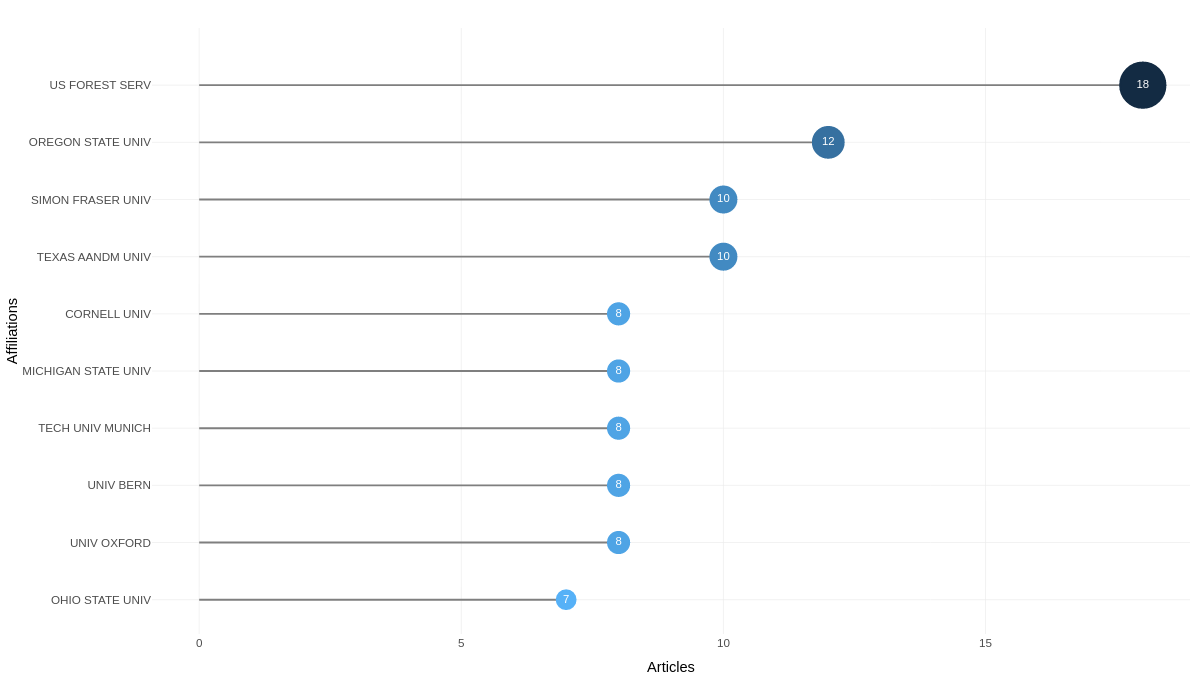
\includegraphics[width=1\textwidth]{exploratory-data-analysis/marcelo3101/PesqBibliogr/ForestFire/WoS-20221204/assets/MostRelevantAffiliationsFFmarcelo3101.png}
    \caption{10 Instituições mais produtivas no tema do \dataset\ FF@marcelo3101, conforme a quantidade de artigos publicados por pessoas a elas filiadas.}
    \label{fig:FF@marcelo3101:Most-Relevant-Affiliations}
\end{figure}

\subsection{Filiações dos autores aos Países}

As instituições às quais são filiados os autores são sediadas em países, o que permite estimar a produtividade e (ou) impacto dos países em um tema de conhecimento específico, como ilustra a tabela \ref{tab:FF@marcelo3101:Most-Cited-Countries}, que mostra a quantidade de citações obtidas pelos artigos das instituições sediadas nesses países.

\begin{table}[htp]
\centering
\resizebox{\textwidth}{!}{%
\begin{tabular}{|l|l|l|}
\hline
Country        & TC   & Average Article Citations \\ \hline
USA            & 3780 & 29.30                     \\ \hline
GERMANY        & 1812 & 86.29                     \\ \hline
CANADA         & 1060 & 31.18                     \\ \hline
SPAIN          & 453  & 56.63                     \\ \hline
AUSTRALIA      & 452  & 32.29                     \\ \hline
ITALY          & 447  & 74.50                     \\ \hline
AUSTRIA        & 411  & 137.00                    \\ \hline
UNITED KINGDOM & 407  & 23.94                     \\ \hline
POLAND         & 288  & 96.00                     \\ \hline
CHINA          & 249  & 10.83                     \\ \hline
\end{tabular}%
}
\caption{10 países com maior impacto de citações no tema do \dataset\ FF@marcelo3101}
\label{tab:FF@marcelo3101:Most-Cited-Countries}
\end{table}

\subsection{Países dos autores principais dos artigos}

Cada artigo escrito por mais de um autor tem um autor responsável por receber as correspondências relativas ao artigo. Esse é o  \textit{wordauthor}. A figura \ref{fig:FF@marcelo3101:Corresponding-Authors-Country} apresenta, em ordem do maior para o menor volume de correspondentes por artigo, o volume publicado por cada país. SCP são as publicações cujos autores são todos do mesmo país. MCP envolve autores de mais de um país.

\begin{figure}
    \centering
    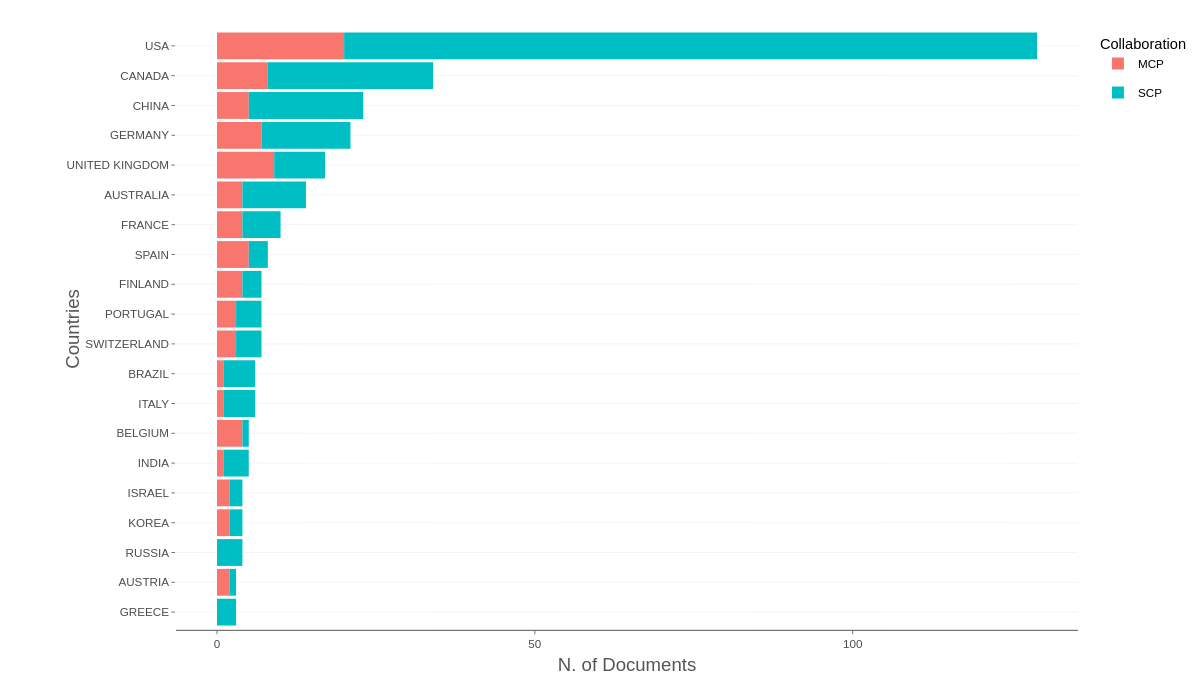
\includegraphics[width=1\textwidth]{exploratory-data-analysis/marcelo3101/PesqBibliogr/ForestFire/WoS-20221204/assets/CorrespondingAuthorsCountryFFmarcelo3101.png}
    \caption{20 principais países que possuem autores responsáveis por receber encomendas por artigos do \dataset\ FF@marcelo3101.}
    \label{fig:FF@marcelo3101:Corresponding-Authors-Country}
\end{figure}

\subsection{Fontes mais relevantes, conforme número de artigos publicados sobre o tema}

Conforme podemos visualizar na figura \ref{fig:FF@marcelo3101:Most-Relevant-Sources}, a fonte mais relevante nesse tema é a revista científica mensal \textit{Ecological Modelling}, se utilizarmos como critério o número de artigos publicados.

\begin{figure}
    \centering
    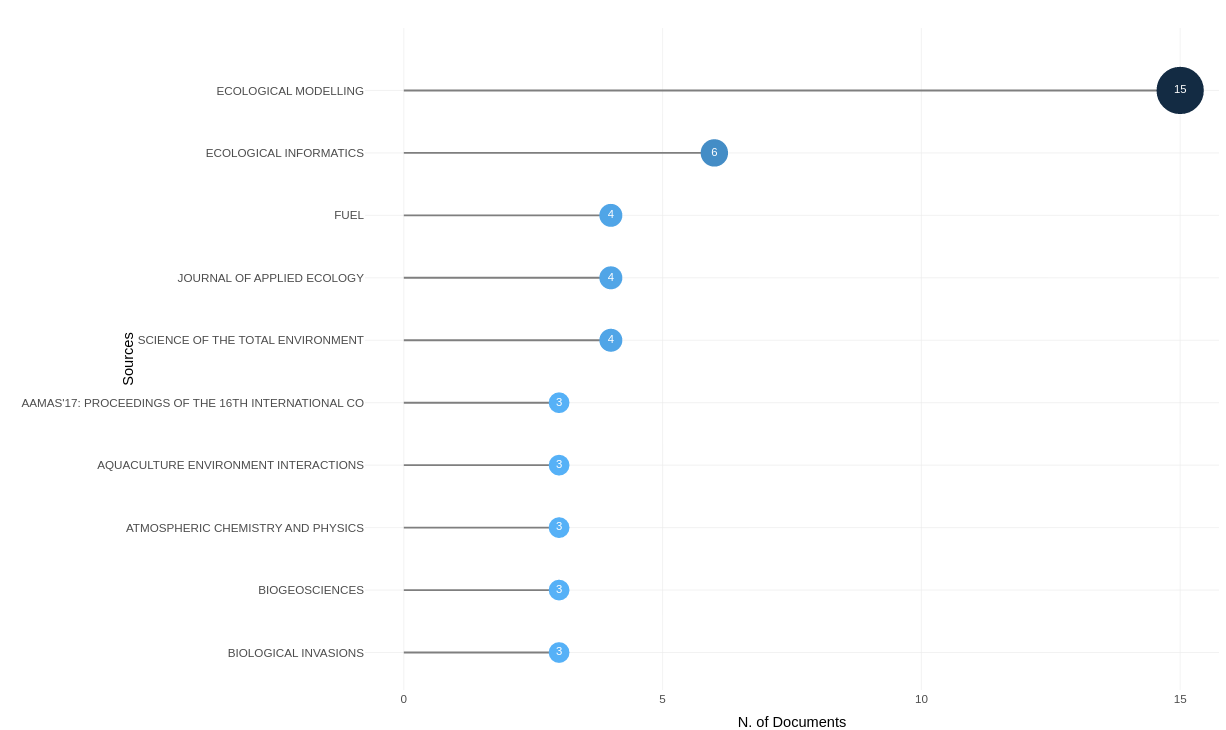
\includegraphics[width=1\textwidth]{exploratory-data-analysis/marcelo3101/PesqBibliogr/ForestFire/WoS-20221204/assets/mostRelevantSourcesFFmarcelo3101.png}
    \caption{Revistas mais relevantes no  \dataset\ FF@marcelo3101.}
    \label{fig:FF@marcelo3101:Most-Relevant-Sources}
\end{figure}

\subsection{Fontes mais relevantes, conforme o número de citações na lista de referências locais}

Conforme podemos visualizar na figura \ref{fig:FF@marcelo3101:Most-Local-Cited-Sources(from-Reference-Lists).png}, a fonte mais relevante nesse tema é a revista semestral \textit{Forest Ecology and Management}, se utilizarmos como critério o número de citações na lista de referências locais.

\begin{figure}
    \centering
    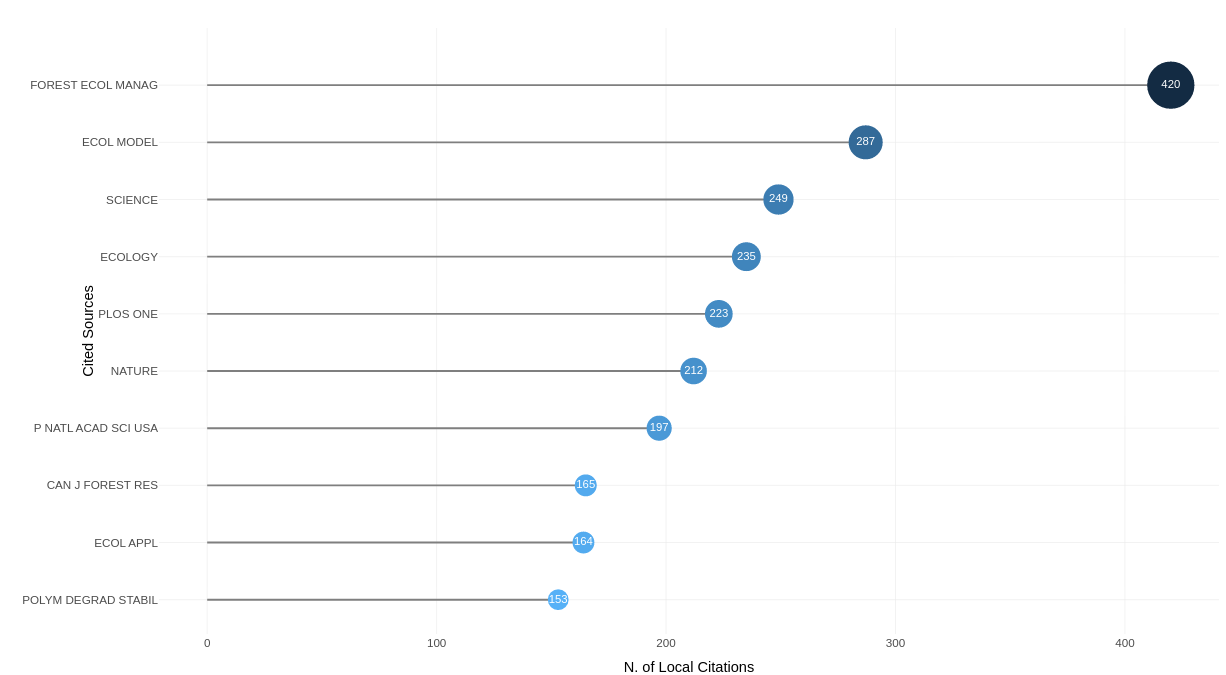
\includegraphics[width=1\textwidth]{exploratory-data-analysis/marcelo3101/PesqBibliogr/ForestFire/WoS-20221204/assets/MostLocalCitedSourcesFFmarcelo3101.png}
    \caption{Revistas mais relevantes no  \dataset\ FF@marcelo3101, conforme a soma de citações aos artigos no \dataset.}
    \label{fig:FF@marcelo3101:Most-Local-Cited-Sources(from-Reference-Lists).png}
\end{figure}

\subsection{Lei de Bradford}

Conforme podemos visualizar na figura \ref{fig:FF@marcelo3101:Bradfords-Law.png}, a fonte mais relevante nesse tema é a revista \textit{Ecological Modelling}, se utilizarmos como critério a Lei de Bradford.

\begin{figure}
    \centering
    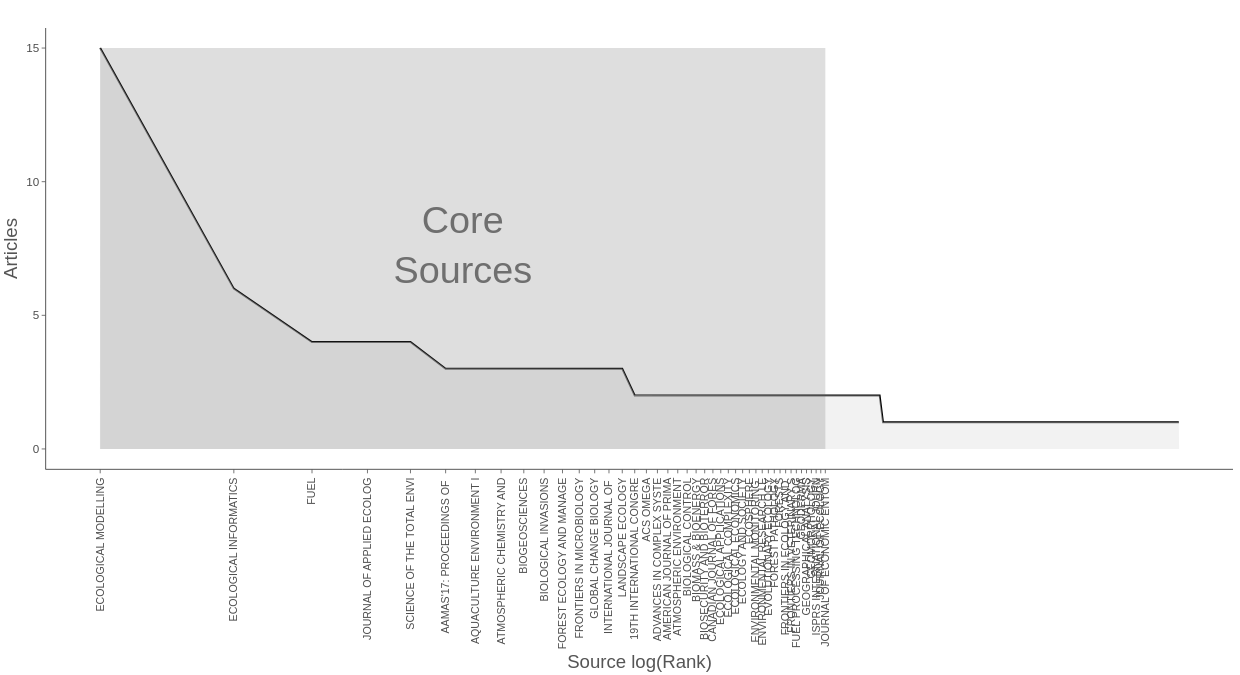
\includegraphics[width=1\textwidth]{exploratory-data-analysis/marcelo3101/PesqBibliogr/ForestFire/WoS-20221204/assets/bradfordsLawFFmarcelo3101.png}
    \caption{Revistas mais relevantes no  \dataset\ FF@marcelo3101, conforme a Lei de Bradford.}
    \label{fig:FF@marcelo3101:Bradfords-Law.png}
\end{figure}

\subsection{Medidas de Impacto das fontes}

Os já apresentados índices H, G e M também podem ser utilizados para medir a relevância das fontes:

\subsubsection{Índice H}

O índice H indica que a revista de maior impacto é a \textit{Ecological Modelling}, conforme mostra a figura \ref{fig:FF@marcelo3101:H-Index-Source-Local-Impact.png}.

\begin{figure}
    \centering
    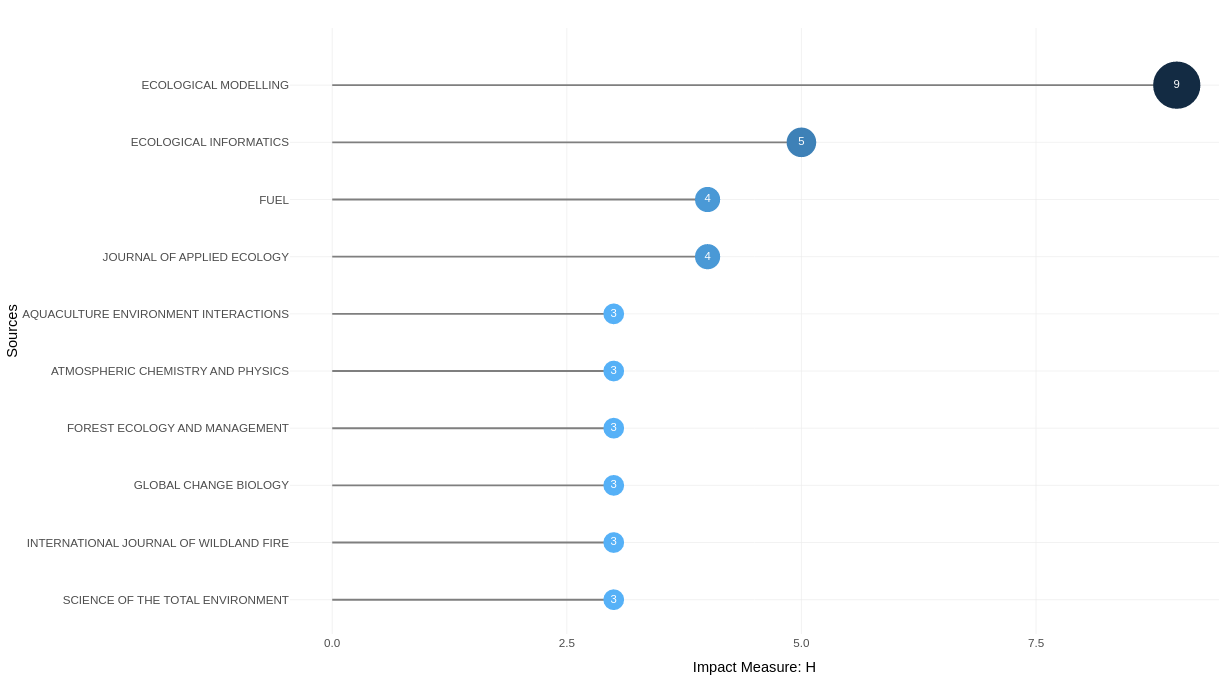
\includegraphics[width=1\textwidth]{exploratory-data-analysis/marcelo3101/PesqBibliogr/ForestFire/WoS-20221204/assets/SourceImpactHindex.png}
    \caption{Revistas de maior impacto no  \dataset\ FF@marcelo3101,  conforme o índice H.}
    \label{fig:FF@marcelo3101:H-Index-Source-Local-Impact.png}
\end{figure}


\subsubsection{Índice G}

O índice G indica que a revista de maior impacto também é a \textit{Ecological Modelling}, conforme mostra a figura \ref{fig:FF@marcelo3101:G-Index-Source-Local-Impact.png}.

\begin{figure}
    \centering
    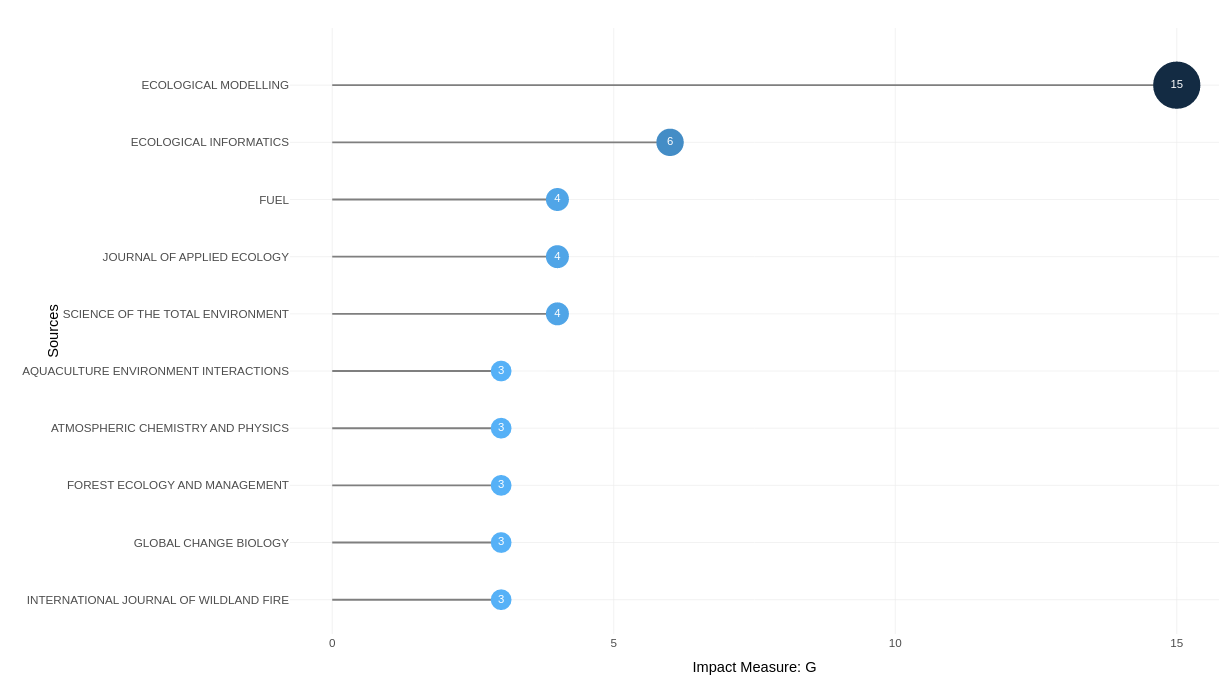
\includegraphics[width=1\textwidth]{exploratory-data-analysis/marcelo3101/PesqBibliogr/ForestFire/WoS-20221204/assets/SourceImpactGindex.png}
    \caption{Revistas de maior impacto no  \dataset\ FF@marcelo3101,  conforme o índice G.}
    \label{fig:FF@marcelo3101:G-Index-Source-Local-Impact.png}
\end{figure}

\subsubsection{Índice M}

O índice M indica fontes empatadas, conforme mostra a figura \ref{fig:FF@marcelo3101:M-Index-Source-Local-Impact.png}.

\begin{figure}
    \centering
    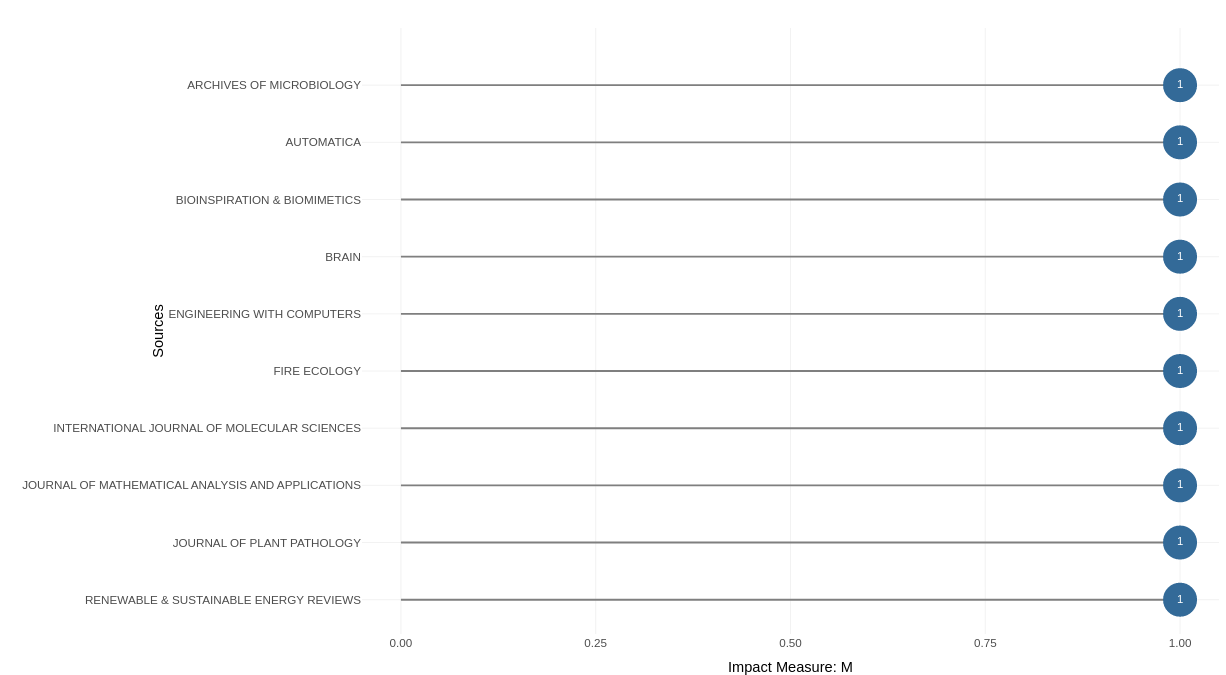
\includegraphics[width=1\textwidth]{exploratory-data-analysis/marcelo3101/PesqBibliogr/ForestFire/WoS-20221204/assets/SourceImpactMindex.png}
    \caption{Revistas de maior impacto no  \dataset\ FF@marcelo3101,  conforme o índice M.}
    \label{fig:FF@marcelo3101:M-Index-Source-Local-Impact.png}
\end{figure}

\subsection{Dinâmica de publicação nas fontes}

E à partir da figura \ref{fig:FF@marcelo3101:Source-Dynamics.png}, podemos visualizar quais revistas tiveram o maior volume de publicações no tema ao longo do tempo.

\begin{figure}
    \centering
    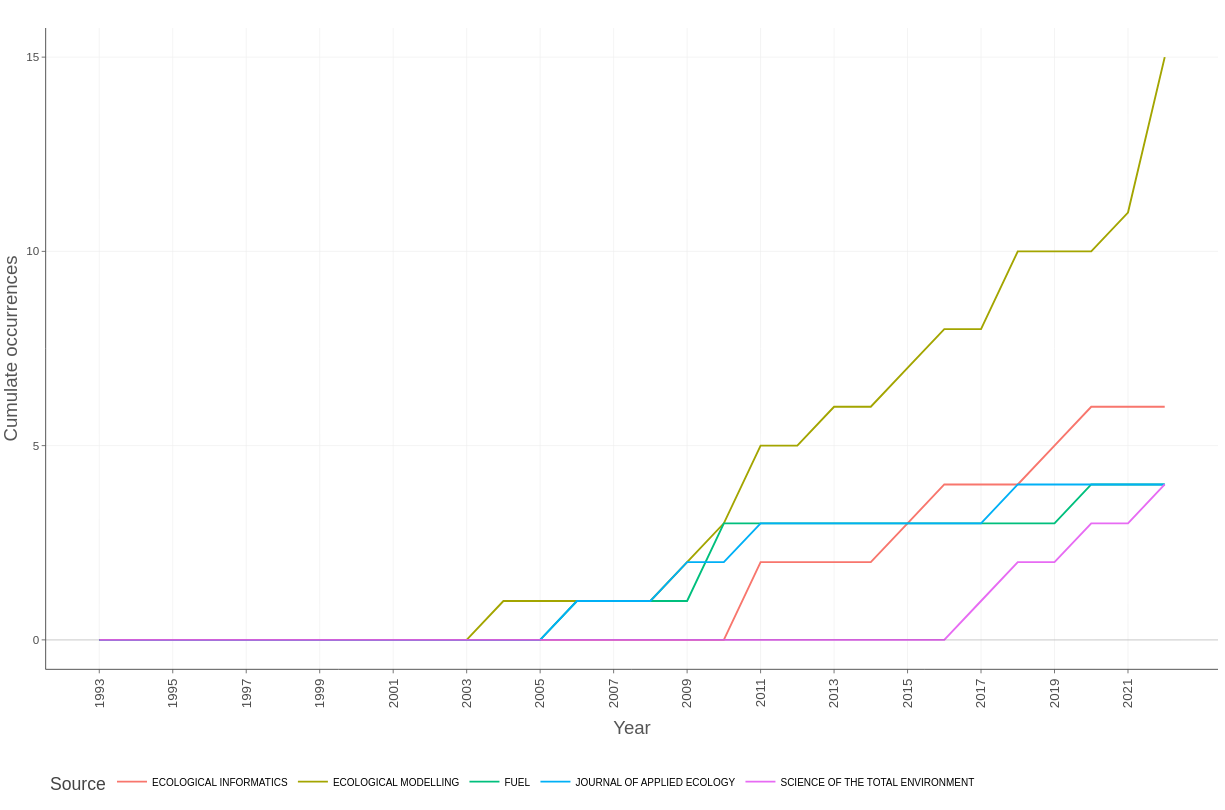
\includegraphics[width=1\textwidth]{exploratory-data-analysis/marcelo3101/PesqBibliogr/ForestFire/WoS-20221204/assets/SourceDynamics.png}
    \caption{Revistas com maior volume de publicações no tema no  \dataset\ FF@marcelo3101, ao longo do tempo.}
    \label{fig:FF@marcelo3101:Source-Dynamics.png}
\end{figure}

\subsection{Estrutura Conceitual do Conhecimento}

O Conhecimento científico é um fenômeno complexo que emerge a partir da agregação memética de termos e palavras, que representam conceitos e ideias, que se organizam em tópicos, temas, e que evoluem ao longo do tempo (ver \url{https://en.wikipedia.org/wiki/Memetics}).

A estrutura conceitual do conhecimento pode ser produzida pela análise de relacionamento estabelecidos entre esses termos. O bibliometrix apresenta um conjunto de técnicas para evidenciar essa estrutura conceitual, e que se organizam em dois grupos:
\begin{description}
    \item [Métricas em rede] que usam grafos para representar relacionamentos entre termos, evidenciando, por meio de métricas de análise de redes sociais, como o conhecimento conceitualmente se organiza.
    \item [Análise Fatorial] Que emprega métricas de redução da dimensionalidade, para explorar, usualmente em mapas bidimensionais, como os termos e palavras se relacionam. 
\end{description}

\subsubsection{Métricas aplicadas a grafos (redes)}

\paragraph{Redes de Coocorrências}

As redes de coocorrências apresentam importantes padrões que se formam nas publicações, e podem revelar a estrutura conceitual de uma área do conhecimento.

No Biblioshiny três tipos de redes podem ser geradas baseadas em coocorrência:
\begin{itemize}
    \item Rede de palavras-chave, revelando quais são as palavras-chave mais comumente usadas simultaneamente em um documento, revelando os grupos de conceitos-chave. As palavras-chave podem ser as originalmente usadas pelos autores (mais variáveis) ou as usadas durante a indexação (mais padronizadas);
    \item Redes de palavras (ngramas) usadas de forma simultânea nos títulos dos artigos;
    \item Redes de palavras (ngramas) usadas de forma simultânea nos resumos dos artigos.
\end{itemize}

A figura \ref{fig:FF@marcelo3101:Co-occurrence-Network} apresenta as 50 palavras-chave padronizadas (Keyword Plus) mais evidentes, clusterizadas pela coocorrência em documentos, no  \dataset\ FF@marcelo3101.

\begin{figure}
    \centering
    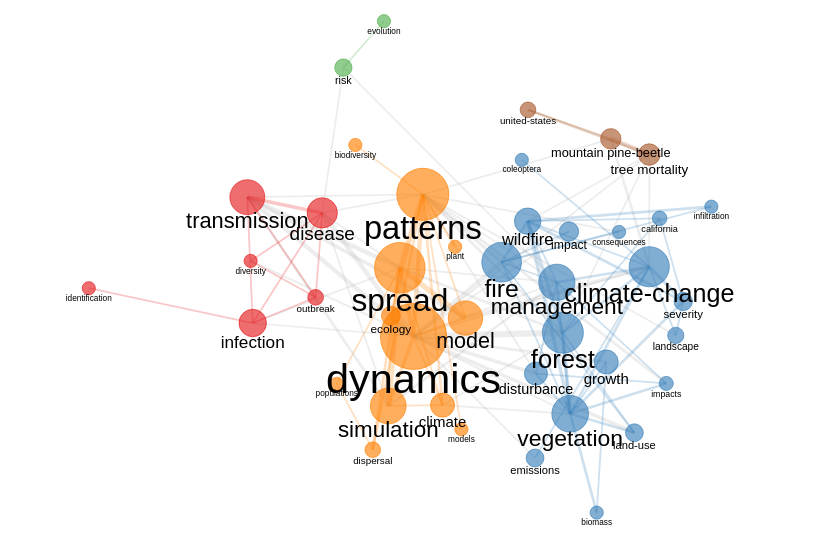
\includegraphics[width=1\textwidth]{exploratory-data-analysis/marcelo3101/PesqBibliogr/ForestFire/WoS-20221204/assets/CooccurenceNetwork.png}
    \caption{50 palavras-chave mais evidentes, clusterizadas pela coocorrência em documentos, no  \dataset\ FF@marcelo3101.}
    \label{fig:FF@marcelo3101:Co-occurrence-Network}
\end{figure}

\paragraph{Mapas Temáticos}

O mapa temático pode ser visualizado na figura \ref{fig:FF@marcelo3101:ThematicMap}. Podemos observar que há temas relacionados a nossa pesquisa como o cluster em azul que envolve dinâmicas de incêndios e o cluster em rosa sobre modelos de \textit{forest-fire}.

\begin{figure}
    \centering
    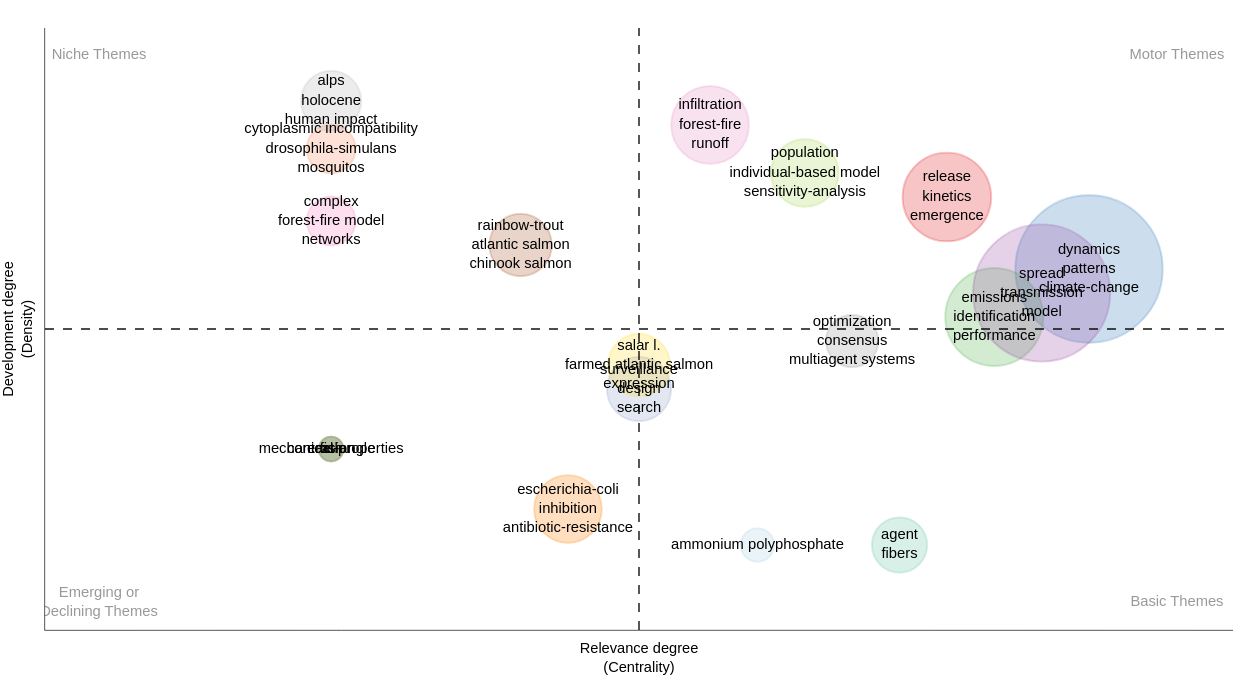
\includegraphics[width=0.9\textwidth]{exploratory-data-analysis/marcelo3101/PesqBibliogr/ForestFire/WoS-20221204/assets/ThematicMap.png}
    \caption{Mapa temático do  \dataset\ FF@marcelo3101.}
    \label{fig:FF@marcelo3101:ThematicMap}
\end{figure}

\paragraph{Evolução Temática}

A evolução temática pode ser visualizada na figura \ref{fig:FF@marcelo3101:Thematic-Evolution}. Podemos observar que grande parte do foco temático se voltou para a estudo de dinâmicas.

\begin{figure}
    \centering
    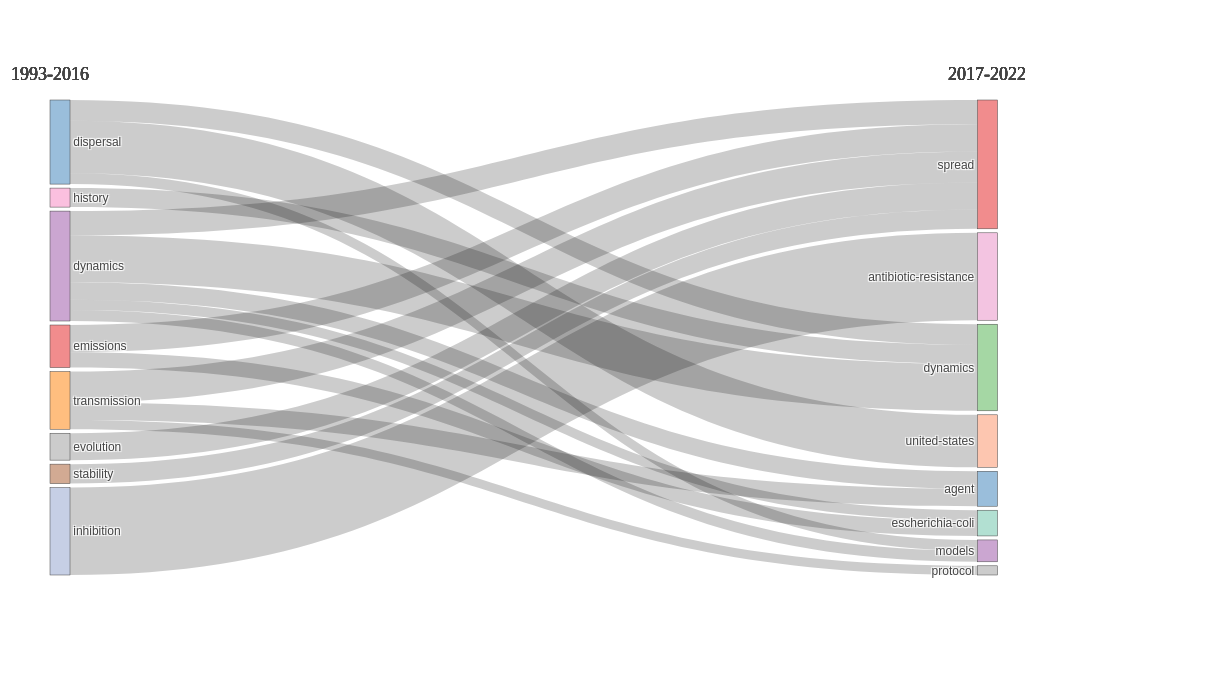
\includegraphics[width=1\textwidth]{exploratory-data-analysis/marcelo3101/PesqBibliogr/ForestFire/WoS-20221204/assets/ThematicEvolution.png}
    \caption{Evolução temática do  \dataset\ FF@marcelo3101.}
    \label{fig:FF@marcelo3101:Thematic-Evolution}
\end{figure}

\subsubsection{Métricas de redução da dimensionalidade (Análise Fatorial)}

No mapa fatorial da figura \ref{fig:FF@marcelo3101:FactorialAnalysis-MCA-FactorialMap}, podemos observar as duas dimensões de temas de estudo.

\begin{figure}
    \centering
    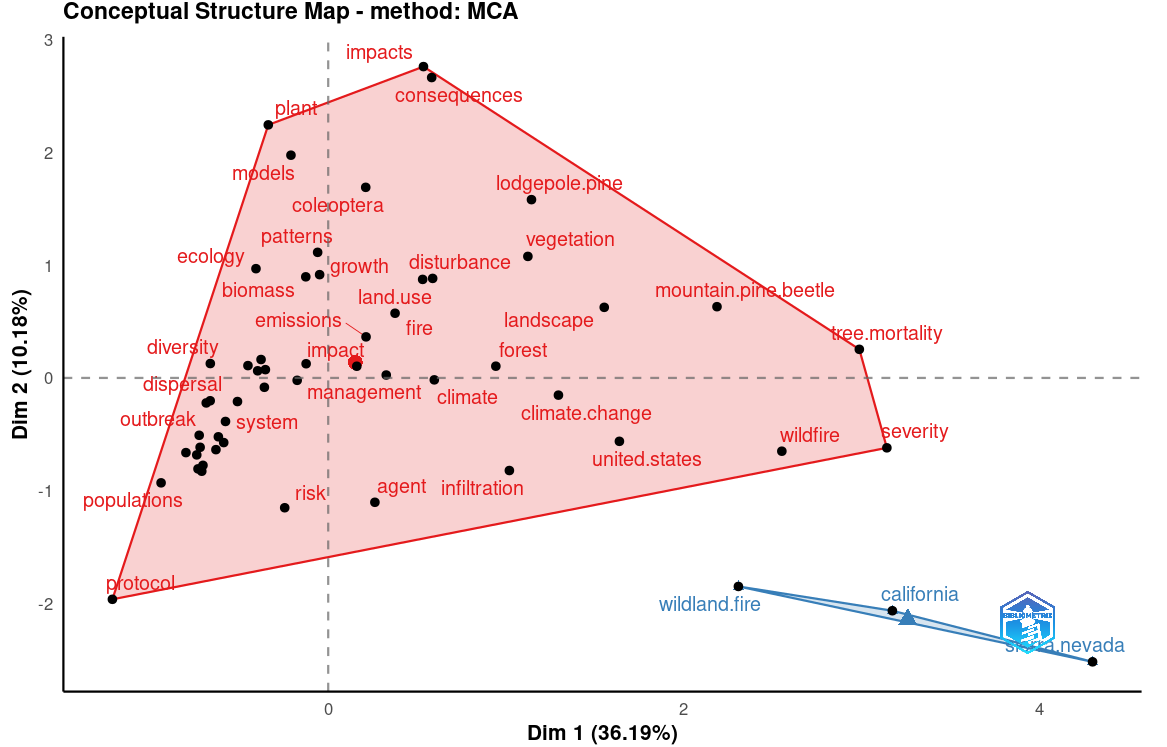
\includegraphics[width=0.9\textwidth]{exploratory-data-analysis/marcelo3101/PesqBibliogr/ForestFire/WoS-20221204/assets/FactorialAnalysis.png}
    \caption{Dimensões de variabilidade mais relevantes, nas palavras-chave do  \dataset\ FF@marcelo3101.}
    \label{fig:FF@marcelo3101:FactorialAnalysis-MCA-FactorialMap}
\end{figure}

\subsection{Estrutura Intelectual do Conhecimento}

Conhecimento científico é produzido por processos intelectuais onde autores de trabalho escolhem deliberadamente referenciar trabalhos de outros, por meio de documentos publicados, que são encaminhados para publicações em fontes de informação de sua escolha, e que evoluem ao longo do tempo.

O Bibliometrix permite exploração da estrutura intelectual do conhecimento, usando basicamente duas abordagens:
\begin{itemize}
    \item Redes de Co-Citação, abordagem bastante comum;
    \item Historiografia, abordagem pouco usual.
\end{itemize}

\subsubsection{Redes de Co-Citação}

As redes de co-citação entre as referências mais presentes podem ser vistas na figura \ref{fig:FF@marcelo3101:CoCitation-Network}.

\begin{figure}
    \centering
    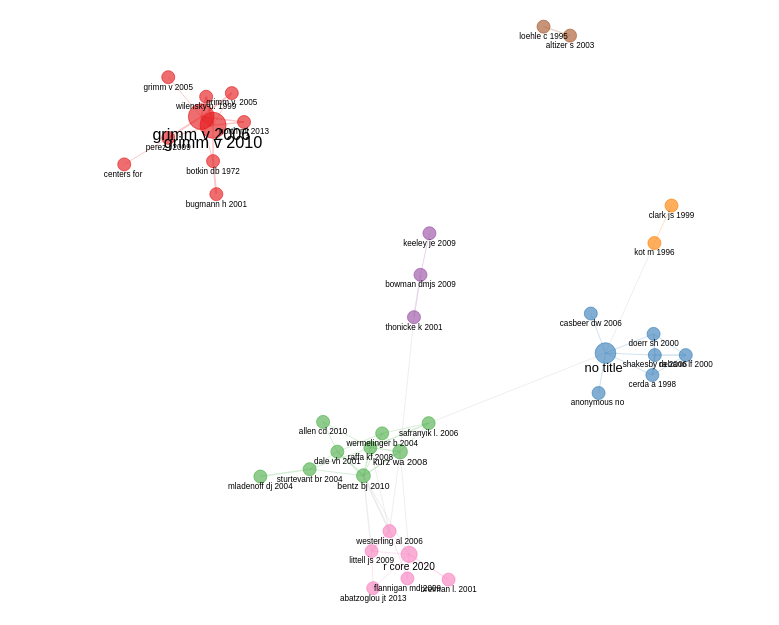
\includegraphics[width=1\textwidth]{exploratory-data-analysis/marcelo3101/PesqBibliogr/ForestFire/WoS-20221204/assets/CocitationNetwork.png}
    \caption{Rede de co-citação entre as 50 referências mais presentes no  \dataset\ FF@marcelo3101.}
    \label{fig:FF@marcelo3101:CoCitation-Network}
\end{figure}

\subsubsection{Historiografia}

O mapa histórico das citações diretas entre os documentos mais evidentes pode ser visto na figura \ref{fig:FF@marcelo3101:HistoricalDirectCitationNetwork-50docs}.

\begin{figure}
    \centering
    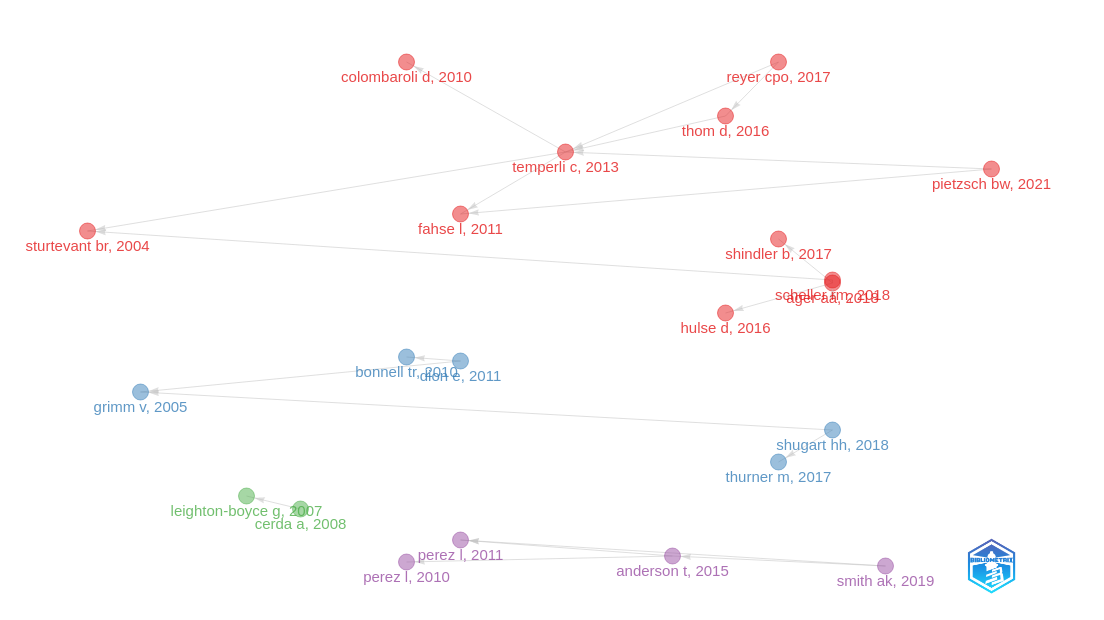
\includegraphics[width=1\textwidth]{exploratory-data-analysis/marcelo3101/PesqBibliogr/ForestFire/WoS-20221204/assets/Historiograph.png}
    \caption{Mapa histórico das citações diretas entre os documentos mais evidentes no  \dataset\ FF@marcelo3101.}
    \label{fig:FF@marcelo3101:HistoricalDirectCitationNetwork-50docs}
\end{figure}

\subsection{Estrutura Social do Conhecimento}

Conhecimento científico é produzido socialmente, por meio de autores trabalhando em conjunto, e uma estrutura de filiações a organizações permanentes ou periódicas, que realizam ou promovem pesquisas, nelas incluídos os centros de pesquisa, universidades, departamentos, institutos, faculdades, eventos, revistas, conferências, e que evoluem ao longo do tempo. A análise da estrutura social do conhecimento evidencia esses relacionamentos, que iniciam no plano pessoal, e evoluem para outros escopos.

\subsubsection{Rede de Colaboração}

As redes de colaboração entre instituições, autores e países podem ser visualizadas nas figuras \ref{fig:FF@marcelo3101:Collaboration-Network-50instit}, \ref{fig:FF@marcelo3101:Collaboration-Network-50authors} e \ref{fig:FF@marcelo3101:Collaboration-Network-50country}, respectivamente. Podemos notar grande colaboração entre instituições norte americanas. E contribuições entre Estados Unidos, Canada, China e países europeus. Alguns países se isolam e se relacionam diretamente com apenas um outro.

\begin{figure}
    \centering
    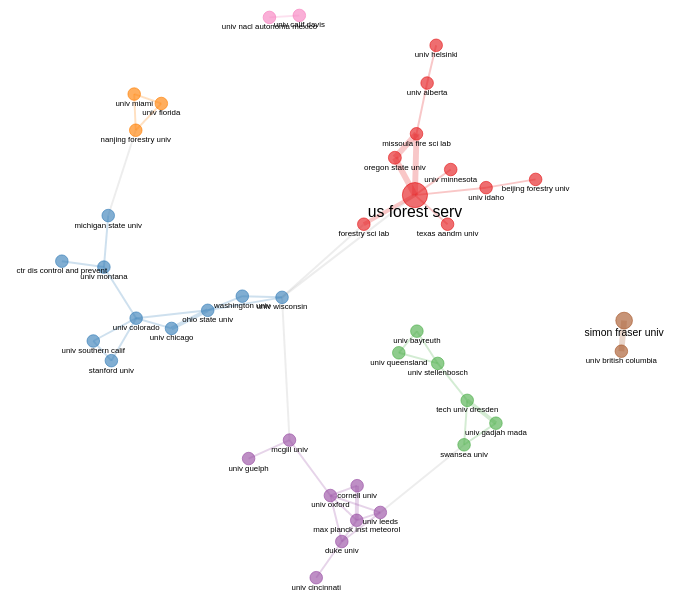
\includegraphics[width=1\textwidth]{exploratory-data-analysis/marcelo3101/PesqBibliogr/ForestFire/WoS-20221204/assets/CollabInst.png}
    \caption{Rede de colaboração entre as 50 instituições mais evidentes, no  \dataset\ FF@marcelo3101.}
    \label{fig:FF@marcelo3101:Collaboration-Network-50instit}
\end{figure}

\begin{figure}
    \centering
    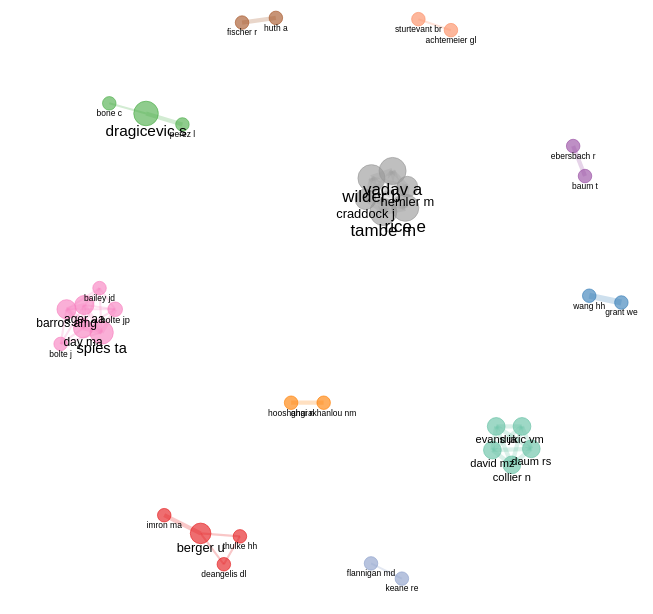
\includegraphics[width=1\textwidth]{exploratory-data-analysis/marcelo3101/PesqBibliogr/ForestFire/WoS-20221204/assets/CollabAuthors.png}
    \caption{Rede de colaboração entre os 50 autores mais evidentes, no  \dataset\ FF@marcelo3101.}
    \label{fig:FF@marcelo3101:Collaboration-Network-50authors}
\end{figure}

\begin{figure}
    \centering
    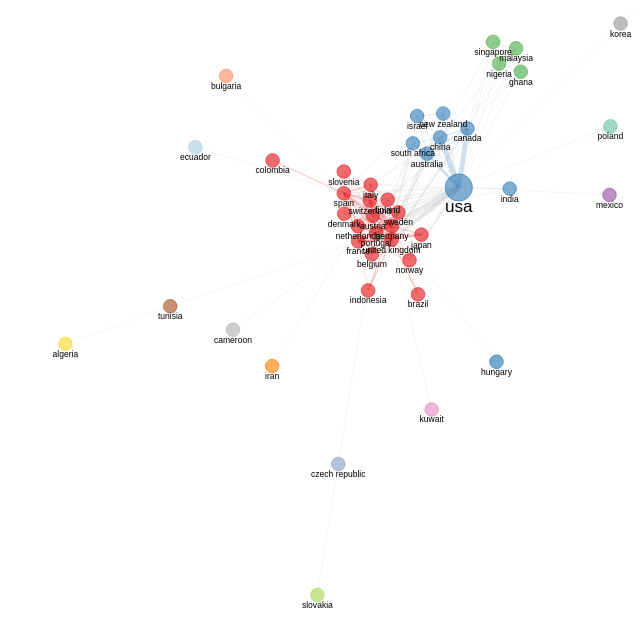
\includegraphics[width=1\textwidth]{exploratory-data-analysis/marcelo3101/PesqBibliogr/ForestFire/WoS-20221204/assets/CollabCountries.png}
    \caption{Rede de colaboração entre os 50 países mais evidentes, no  \dataset\ FF@marcelo3101.}
    \label{fig:FF@marcelo3101:Collaboration-Network-50country}
\end{figure}

\section{Análises\label{FF@marcelo3101:Analises}}

Julgando pela figura \ref{fig:FF@marcelo3101:FactorialAnalysis-MCA-FactorialMap}, na página \pageref{fig:FF@marcelo3101:FactorialAnalysis-MCA-FactorialMap}, ver que vários temas são estudados, separados em duas dimensões. No entanto, ao analisarmos de perto quais são os termos que definem essas áreas, podemos observar que as pesquisas na área representada pelo polígono azul possuem foco em casos de incêndios reais. 

A área de pesquisa ilustrada pelo polígono vermelho estuda muitos outros fenômenos relacionados ao tema, como os impactos causados, consequências, mudança climática, risco e modelos de forest-fire.

Com relação ao uso de simulações, podemos observar que elas são utilizadas para descrever e entender os possíveis padrões de comportamento da ignição e dispersão do fogo nessas regiões. Além de avaliar o risco e mortalidade de árvores. As simulações atingem esses objetivos ao usarem modelos de simulação \textit{forest-fire}.

\section{Conclusões}

Este trabalho está apresenta o arcabouço geral de informações que possibilitam responder às  questões formuladas no início da pesquisa, em \ref{FF@marcelo3101:questoes}:

\subsection{Base de conhecimentos}

O que pode se dizer sobre a produção científica global acerca desse assunto específico?? 
 
Resposta: Ver, em \ref{fig:evol:anual:FF@marcelo3101} que o número de artigos tem uma taxa de crescimento alta, que indica uma produção contínua sobre o tema abordado.

\subsection{Fenômenos}
   
Como a simulação multiagente tem sido usada para compreender os fenômenos de ignição e espalhamento do fogo envolvidos nesses incêndios?

Resposta: Ver \ref{FF@marcelo3101:Analises}.

\subsection{Termos e conceitos centrais}

Quais são os principais conceitos ligados ao tema de pesquisa sobre incêndios florestais? 

Resposta: Ver e explorar os mapas das figuras \ref{fig:FF@marcelo3101:Co-occurrence-Network}, \ref{fig:FF@marcelo3101:ThematicMap}, entre outros.

\subsection{Estrutura Social da Comunidade}

Quais países que se destacam na pesquisa sobre simulações de incêndios florestais?

Resposta: Ver e analisar os mapas das figuras \ref{fig:FF@marcelo3101:Collaboration-Network-50authors}, \ref{fig:FF@marcelo3101:Collaboration-Network-50instit} e \ref{fig:FF@marcelo3101:Collaboration-Network-50country}, a tabela \ref{tab:FF@marcelo3101:Most-Cited-Countries}. Além da figura \ref{fig:FF@marcelo3101:Corresponding-Authors-Country}. 
